%!TEX root = ../chapter2.tex
% ******************************* Thesis Appendix A ****************************
\chapter{}

\begin{figure}[h]
 \centering
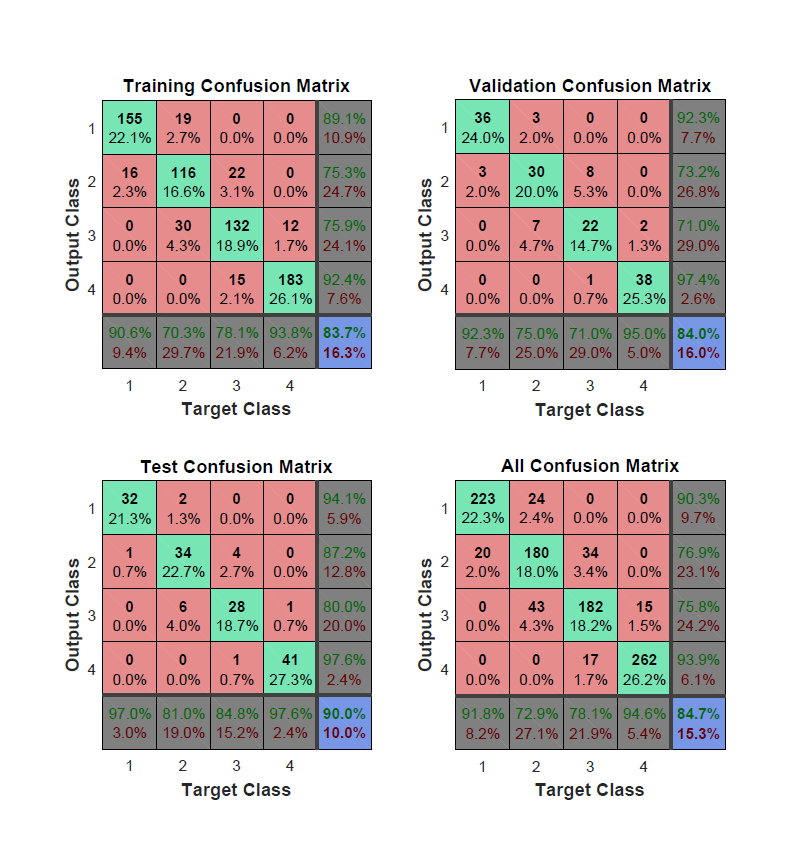
\includegraphics[width=0.5\textwidth]{Chapter2/2002_CM_Fev_MA.png}
\caption[Confusion Matrix Results for 2002 in Cerrado Maranhao]{Confusion Matrix Results for 2002 in Cerrado Maranhao. Final confusion matrix is at the bottom right. The rows correspond to the predicted class and the columns correspond to the true class. The diagonal cells correspond to observations that are correctly classified. Both the number of observations and the percentage of the total number of observations are shown in each cell. The column on the far right of the plot shows the percentages of all the examples predicted to belong to each class that are correctly and incorrectly classified. The row at the bottom of the plot shows the percentages of all the examples belonging to each class that are correctly and incorrectly classified. The cell in the bottom right of the plot shows the overall accuracy \citep{matlab_2017}.}
\end{figure}


\begin{figure}[htpb]
 \centering
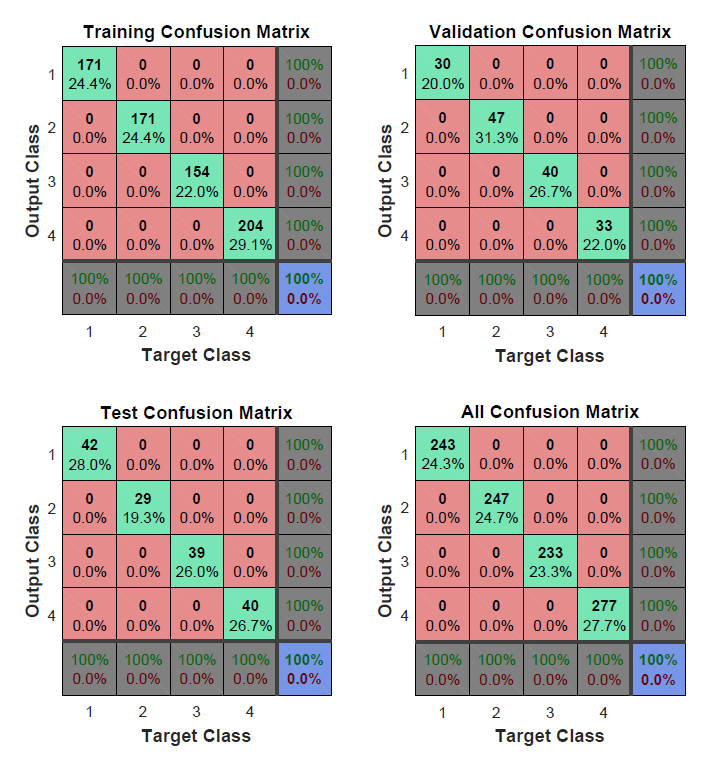
\includegraphics[width=0.9\textwidth]{Chapter2/2002_CM_Fev_ML_N.png}
\caption[Confusion Matrix Results for 2002 in Legal Maranhao]{Confusion Matrix Results for 2002 in Legal Maranhao. Final confusion matrix is at the bottom right. The rows correspond to the predicted class and the columns correspond to the true class. The diagonal cells correspond to observations that are correctly classified. Both the number of observations and the percentage of the total number of observations are shown in each cell. The column on the far right of the plot shows the percentages of all the examples predicted to belong to each class that are correctly and incorrectly classified. The row at the bottom of the plot shows the percentages of all the examples belonging to each class that are correctly and incorrectly classified. The cell in the bottom right of the plot shows the overall accuracy \citep{matlab_2017}.}
\end{figure}

\begin{figure}[htpb]
 \centering
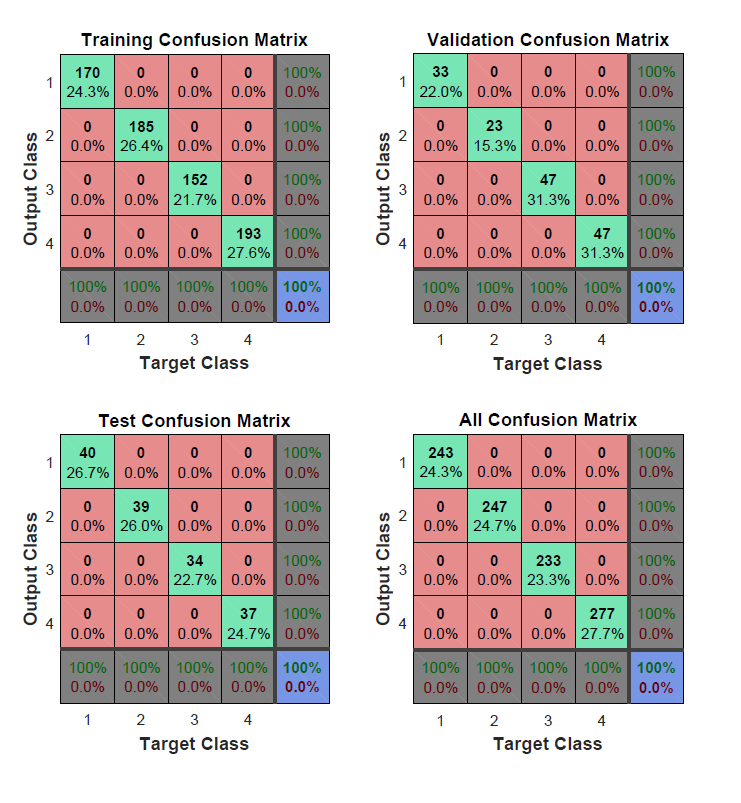
\includegraphics[width=0.9\textwidth]{Chapter2/2005_CM_Mai_MA_N.png}
\caption[Confusion Matrix Results for 2012 in Cerrado Maranhao]{Confusion Matrix Results for 2012 in Cerrado Maranhao. Final confusion matrix is at the bottom right. The rows correspond to the predicted class and the columns correspond to the true class. The diagonal cells correspond to observations that are correctly classified. Both the number of observations and the percentage of the total number of observations are shown in each cell. The column on the far right of the plot shows the percentages of all the examples predicted to belong to each class that are correctly and incorrectly classified. The row at the bottom of the plot shows the percentages of all the examples belonging to each class that are correctly and incorrectly classified. The cell in the bottom right of the plot shows the overall accuracy \citep{matlab_2017}.}
\end{figure}


\begin{figure}[htpb]
 \centering
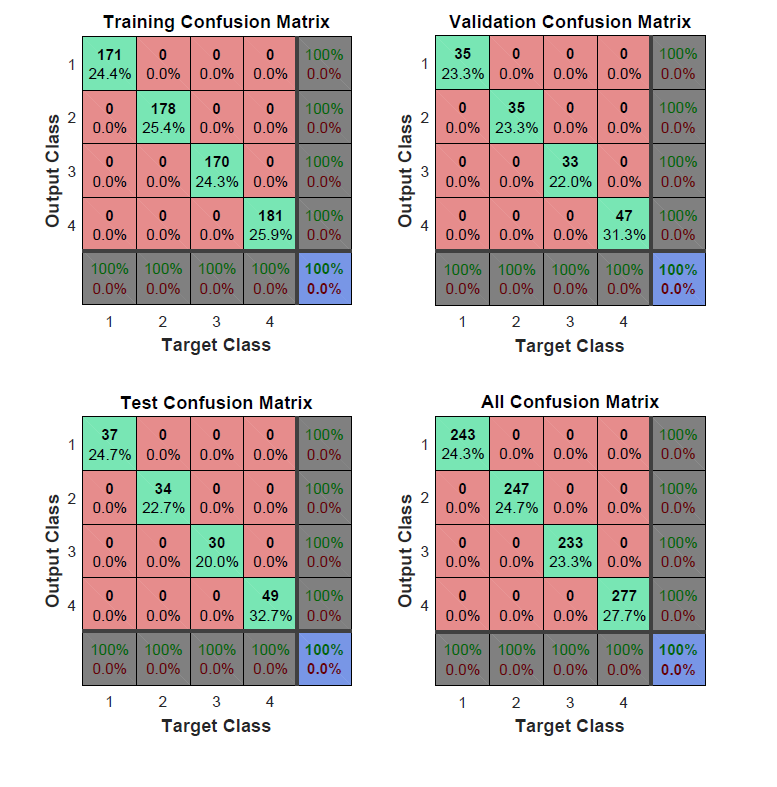
\includegraphics[width=0.9\textwidth]{Chapter2/2005_CM_Mai_ML_N.png}
\caption[Confusion Matrix Results for 2012 in Legal Maranhao]{Confusion Matrix Results for 2012 in Legal Maranhao. Final confusion matrix is at the bottom right. The rows correspond to the predicted class and the columns correspond to the true class. The diagonal cells correspond to observations that are correctly classified. Both the number of observations and the percentage of the total number of observations are shown in each cell. The column on the far right of the plot shows the percentages of all the examples predicted to belong to each class that are correctly and incorrectly classified. The row at the bottom of the plot shows the percentages of all the examples belonging to each class that are correctly and incorrectly classified. The cell in the bottom right of the plot shows the overall accuracy \citep{matlab_2017}.}
\end{figure}

\begin{sidewaystable}
\begin{figure}[H]
 \centering
    %\begin{minipage}{1\textwidth}
        \centering
        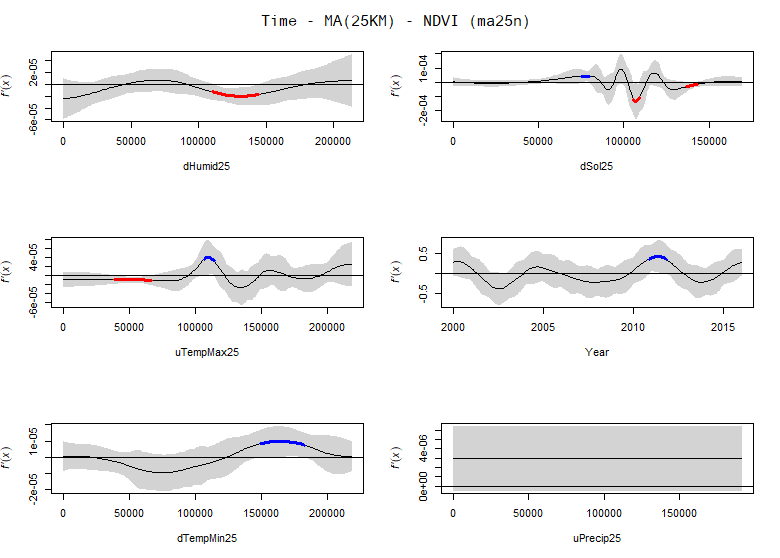
\includegraphics[width=0.8\textwidth]{ma25n.png} % first figure itself
        \caption[Model Cerrado Maranhão for 25km bandwidth using NDVI values. First derivative of the trends splines from the deforestation data Generalized Additive Model (GAM)]{\textbf{Model ma25n}. Model Maranhão Cerrado for 25km bandwidth using NDVI values. First derivative of the trends splines from the deforestation data Generalized Additive Model (GAM). The grey band is a 99\% simultaneous point-wise confidence interval. Sections of the spline where the confidence interval does not include zero are indicated by coloured sections. Blue colour means positive values and red colour means negative values.}
    %\end{minipage}
\end{figure}
\end{sidewaystable}

\begin{sidewaystable}

\begin{figure}[H]
 \centering
    %\begin{minipage}{1\textwidth}
        \centering
        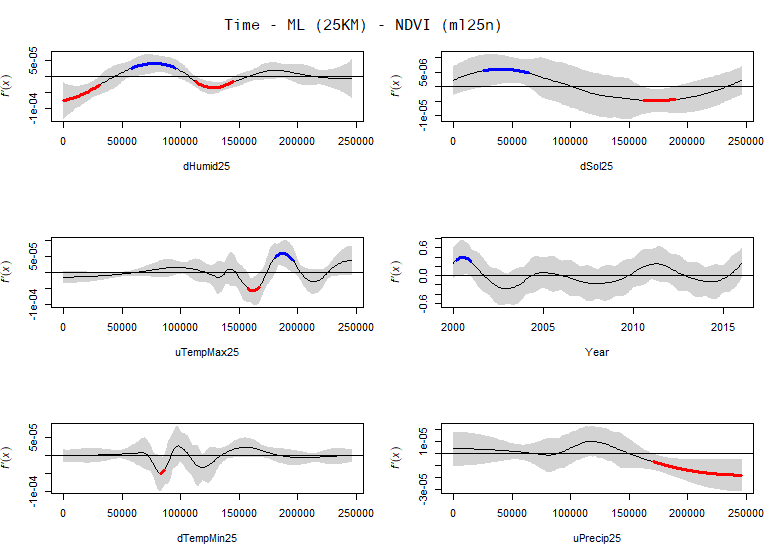
\includegraphics[width=0.8\textwidth]{ml25n.png} % second figure itself
        \caption[Model Legal Maranhão for 25km bandwidth using NDVI values. First derivative of the trends splines from the deforestation data Generalized Additive Model (GAM)]{\textbf{Model lm25n}. Model Legal Maranhão for 25km bandwidth using NDVI values. First derivative of the trends splines from the deforestation data Generalized Additive Model (GAM). The grey band is a 99\% simultaneous point-wise confidence interval. Sections of the spline where the confidence interval does not include zero are indicated by coloured sections. Blue colour means positive values and red colour means negative values.}
        \centering
\end{figure}
\end{sidewaystable}

\begin{sidewaystable}
\begin{figure}[H]
 \centering
    %\begin{minipage}{1\textwidth}
        \centering
        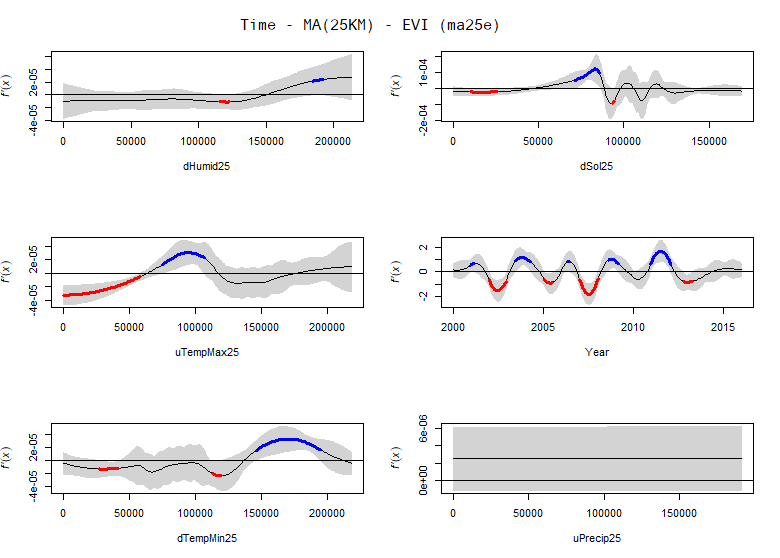
\includegraphics[width=0.8\textwidth]{ma25e.png} % first figure itself
        \caption[Model Cerrado Maranhão for 25km bandwidth using EVI values. First derivative of the trends splines from the deforestation data Generalized Additive Model (GAM)]{\textbf{Model ma25e}. Model Maranhão Cerrado for 25km bandwidth using EVI values. First derivative of the trends splines from the deforestation data Generalized Additive Model (GAM). The grey band is a 99\% simultaneous point-wise confidence interval. Sections of the spline where the confidence interval does not include zero are indicated by coloured sections. Blue colour means positive values and red colour means negative values.}
    %\end{minipage}
\end{figure}
\end{sidewaystable}

\begin{sidewaystable}
\begin{figure}[H]
 \centering
    %\begin{minipage}{1\textwidth}
        \centering
        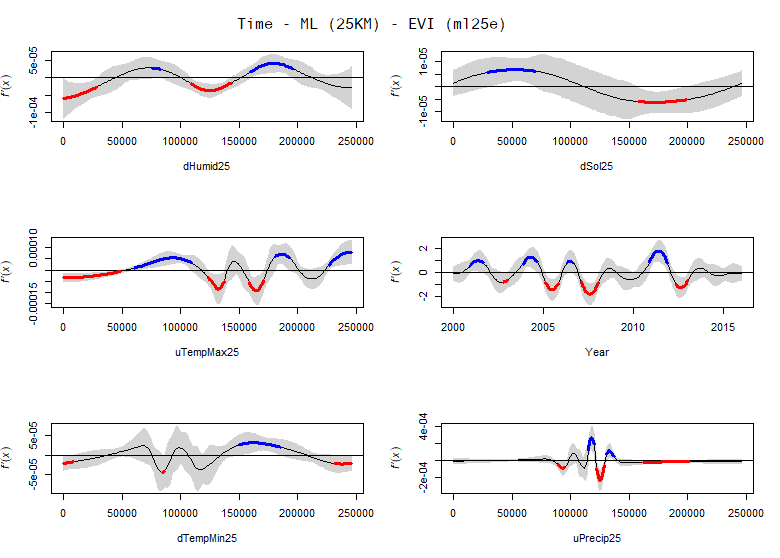
\includegraphics[width=0.8\textwidth]{ml25e.png} % second figure itself
        \caption[Model Legal Maranhão for 25km bandwidth using EVI values. First derivative of the trends splines from the deforestation data Generalized Additive Model (GAM)]{\textbf{Model lm25e}. Model Legal Maranhão for 25km bandwidth using EVI values. First derivative of the trends splines from the deforestation data Generalized Additive Model (GAM). The grey band is a 99\% simultaneous point-wise confidence interval. Sections of the spline where the confidence interval does not include zero are indicated by coloured sections. Blue colour means positive values and red colour means negative values.}
        \centering
\end{figure}
\end{sidewaystable}

%%%%%%%%%%%%%%%%%%%%%%%%%%%%%%%%%%%%%%%%%%%%%%%%%%%%%%%%%%%%%%%%%%%%%%%%%%%%%%%%%%%%%

\begin{sidewaystable}
\begin{figure}[H]
 \centering
    %\begin{minipage}{1\textwidth}
        \centering
        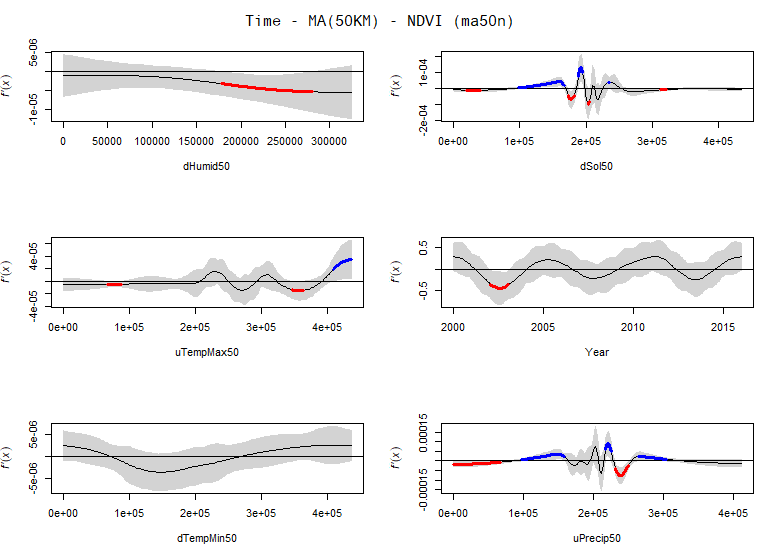
\includegraphics[width=0.8\textwidth]{ma50n.png} % first figure itself
        \caption[Model Cerrado Maranhão for 50km bandwidth using NDVI values. First derivative of the trends splines from the deforestation data Generalized Additive Model (GAM)]{\textbf{Model ma50n}. Model Maranhão Cerrado for 50km bandwidth using NDVI values. First derivative of the trends splines from the deforestation data Generalized Additive Model (GAM). The grey band is a 99\% simultaneous point-wise confidence interval. Sections of the spline where the confidence interval does not include zero are indicated by coloured sections. Blue colour means positive values and red colour means negative values.}
    %\end{minipage}
\end{figure}

\end{sidewaystable}

\begin{sidewaystable}

\begin{figure}[H]
 \centering
    %\begin{minipage}{1\textwidth}
        \centering
        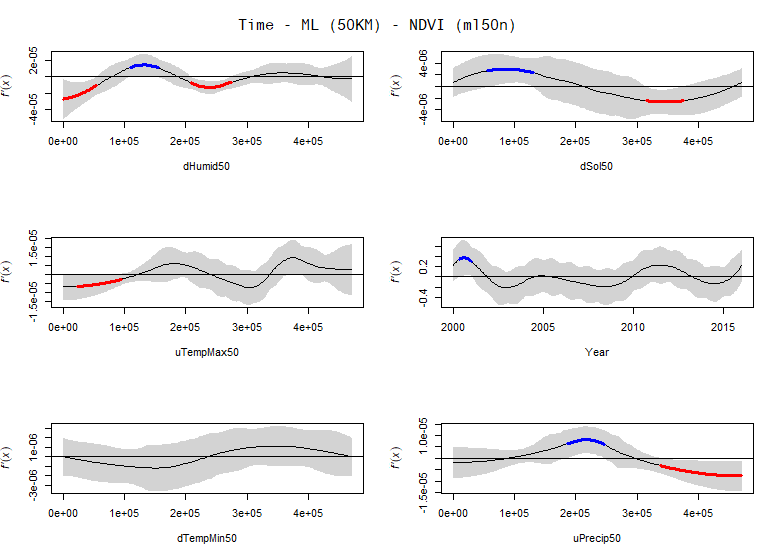
\includegraphics[width=0.8\textwidth]{ml50n.png} % second figure itself
        \caption[Model Legal Maranhão for 50km bandwidth using NDVI values. First derivative of the trends splines from the deforestation data Generalized Additive Model (GAM)]{\textbf{Model lm50n}. Model Legal Maranhão for 50km bandwidth using NDVI values. First derivative of the trends splines from the deforestation data Generalized Additive Model (GAM). The grey band is a 99\% simultaneous point-wise confidence interval. Sections of the spline where the confidence interval does not include zero are indicated by coloured sections. Blue colour means positive values and red colour means negative values.}
        \centering
\end{figure}

\end{sidewaystable}

\begin{sidewaystable}

\begin{figure}[H]
 \centering
    %\begin{minipage}{1\textwidth}
        \centering
        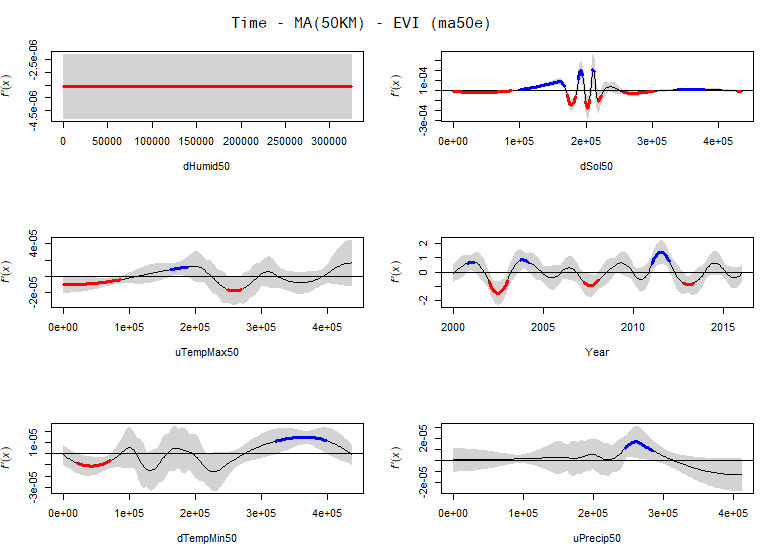
\includegraphics[width=0.8\textwidth]{ma50e.png} % first figure itself
        \caption[Model Cerrado Maranhão for 50km bandwidth using EVI values. First derivative of the trends splines from the deforestation data Generalized Additive Model (GAM)]{\textbf{Model ma50e}. Model Maranhão Cerrado for 50km bandwidth using EVI values. First derivative of the trends splines from the deforestation data Generalized Additive Model (GAM). The grey band is a 99\% simultaneous point-wise confidence interval. Sections of the spline where the confidence interval does not include zero are indicated by coloured sections. Blue colour means positive values and red colour means negative values.}
    %\end{minipage}
\end{figure}
\end{sidewaystable}

\begin{sidewaystable}
\begin{figure}[H]
 \centering
    %\begin{minipage}{1\textwidth}
        \centering
        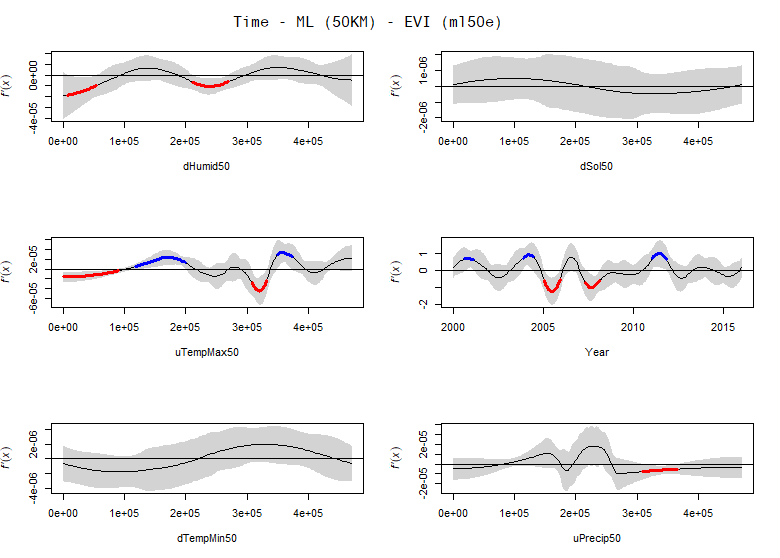
\includegraphics[width=0.8\textwidth]{ml50e.png} % second figure itself
        \caption[Model Legal Maranhão for 50km bandwidth using EVI values. First derivative of the trends splines from the deforestation data Generalized Additive Model (GAM)]{\textbf{Model lm50e}. Model Legal Maranhão for 50km bandwidth using EVI values. First derivative of the trends splines from the deforestation data Generalized Additive Model (GAM). The grey band is a 99\% simultaneous point-wise confidence interval. Sections of the spline where the confidence interval does not include zero are indicated by coloured sections. Blue colour means positive values and red colour means negative values.}
        \centering
\end{figure}

\end{sidewaystable}

%%%%%%%%%%%%%%%%%%%%%%%%%%%%%%%%%%%%%%%%%%%%%%%%%%%%%%%%%%%%%%%%%%%%%%%%%%%%%%%%%%
\begin{sidewaystable}
\begin{figure}[H]
 \centering
    %\begin{minipage}{1\textwidth}
        \centering
        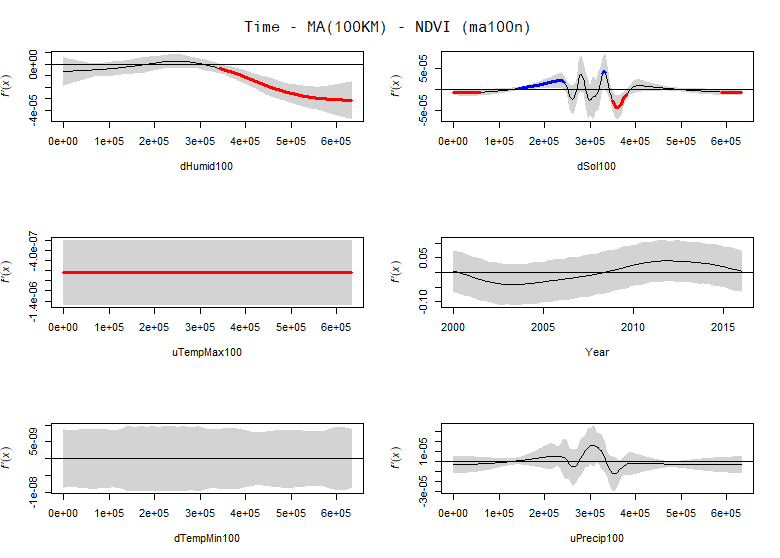
\includegraphics[width=0.8\textwidth]{ma100n.png} % first figure itself
        \caption[Model Cerrado Maranhão for 100km bandwidth using NDVI values. First derivative of the trends splines from the deforestation data Generalized Additive Model (GAM)]{\textbf{Model ma100n}. Model Maranhão Cerrado for 100km bandwidth using NDVI values. First derivative of the trends splines from the deforestation data Generalized Additive Model (GAM). The grey band is a 99\% simultaneous point-wise confidence interval. Sections of the spline where the confidence interval does not include zero are indicated by coloured sections. Blue colour means positive values and red colour means negative values.}
    %\end{minipage}
\end{figure}

\end{sidewaystable}

\begin{sidewaystable}


\begin{figure}[H]
 \centering
    %\begin{minipage}{1\textwidth}
        \centering
        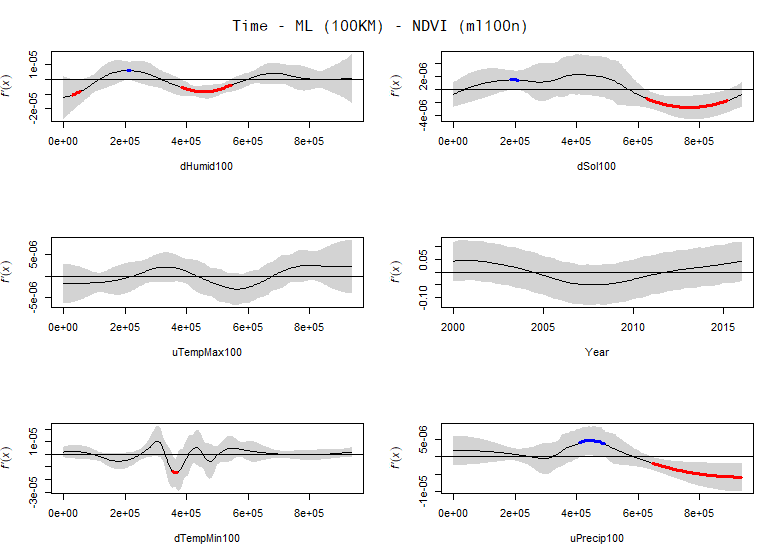
\includegraphics[width=0.8\textwidth]{ml100n.png} % second figure itself
        \caption[Model Legal Maranhão for 100km bandwidth using NDVI values. First derivative of the trends splines from the deforestation data Generalized Additive Model (GAM)]{\textbf{Model lm100n}. Model Legal Maranhão for 100km bandwidth using NDVI values. First derivative of the trends splines from the deforestation data Generalized Additive Model (GAM). The grey band is a 99\% simultaneous point-wise confidence interval. Sections of the spline where the confidence interval does not include zero are indicated by coloured sections. Blue colour means positive values and red colour means negative values.}
        \centering
\end{figure}
\end{sidewaystable}

\begin{sidewaystable}

\begin{figure}[H]
 \centering
    %\begin{minipage}{1\textwidth}
        \centering
        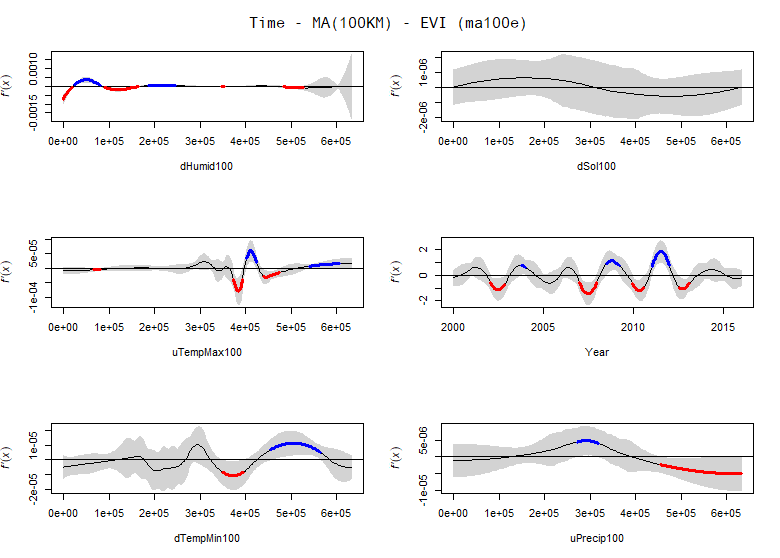
\includegraphics[width=0.8\textwidth]{ma100e.png} % first figure itself
        \caption[Model Cerrado Maranhão for 100km bandwidth using EVI values. First derivative of the trends splines from the deforestation data Generalized Additive Model (GAM)]{\textbf{Model ma100e}. Model Maranhão Cerrado for 100km bandwidth using EVI values. First derivative of the trends splines from the deforestation data Generalized Additive Model (GAM). The grey band is a 99\% simultaneous point-wise confidence interval. Sections of the spline where the confidence interval does not include zero are indicated by coloured sections. Blue colour means positive values and red colour means negative values.}
    %\end{minipage}
\end{figure}
\end{sidewaystable}

\begin{sidewaystable}

\begin{figure}[H]
 \centering
    %\begin{minipage}{1\textwidth}
        \centering
        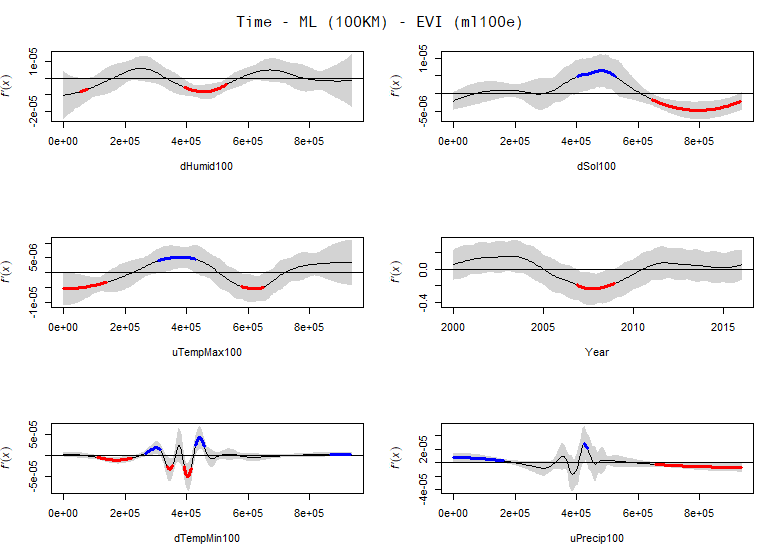
\includegraphics[width=0.8\textwidth]{ml100e.png} % second figure itself
        \caption[Model Legal Maranhão for 100km bandwidth using EVI values. First derivative of the trends splines from the deforestation data Generalized Additive Model (GAM)]{\textbf{Model lm100e}. Model Legal Maranhão for 100km bandwidth using EVI values. First derivative of the trends splines from the deforestation data Generalized Additive Model (GAM). The grey band is a 99\% simultaneous point-wise confidence interval. Sections of the spline where the confidence interval does not include zero are indicated by coloured sections. Blue colour means positive values and red colour means negative values.}
        \centering
\end{figure}
\end{sidewaystable}

%%%%%%%%%%%%%%%%%%%%%%%%%%%%%%%%%%%%%% R A I N I N G %%%%%%%%%%%%%%%%%%%%%%%%%%%%

\begin{sidewaystable}


\begin{figure}[H]
 \centering
    %\begin{minipage}{1\textwidth}
        \centering
        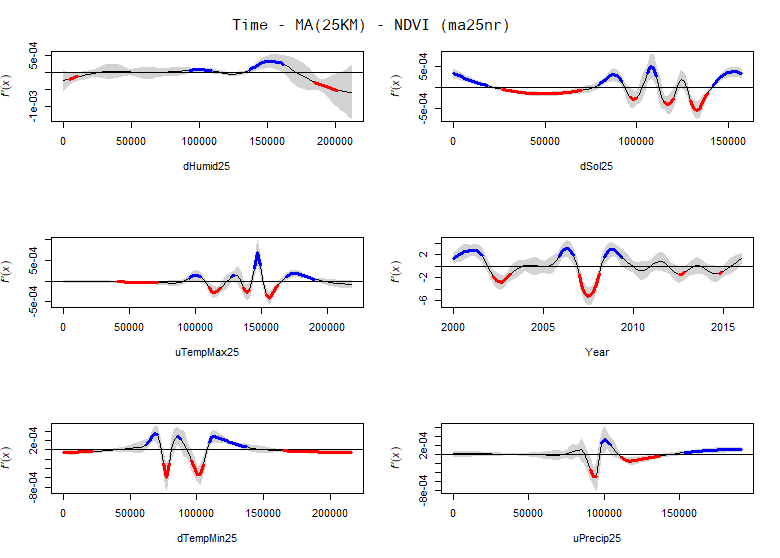
\includegraphics[width=0.8\textwidth]{ma25nr.png} % first figure itself
        \caption[Model Cerrado Maranhão for 25km bandwidth using NDVI values for raining season. First derivative of the trends splines from the deforestation data Generalized Additive Model (GAM)]{\textbf{Model ma25nr}. Model Maranhão Cerrado for 25km bandwidth using NDVI values for raining season. First derivative of the trends splines from the deforestation data Generalized Additive Model (GAM). The grey band is a 99\% simultaneous point-wise confidence interval. Sections of the spline where the confidence interval does not include zero are indicated by coloured sections. Blue colour means positive values and red colour means negative values.}
    %\end{minipage}
\end{figure}
\end{sidewaystable}

\begin{sidewaystable}

\begin{figure}[H]
 \centering
    %\begin{minipage}{1\textwidth}
        \centering
        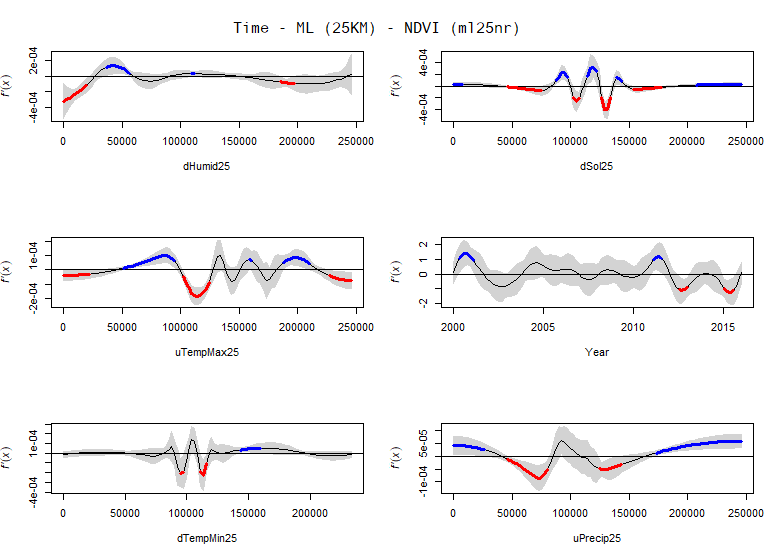
\includegraphics[width=0.8\textwidth]{ml25nr.png} % second figure itself
        \caption[Model Legal Maranhão for 25km bandwidth using NDVI values for raining season. First derivative of the trends splines from the deforestation data Generalized Additive Model (GAM)]{\textbf{Model lm25nr}. Model Legal Maranhão for 25km bandwidth using NDVI values for raining season. First derivative of the trends splines from the deforestation data Generalized Additive Model (GAM). The grey band is a 99\% simultaneous point-wise confidence interval. Sections of the spline where the confidence interval does not include zero are indicated by coloured sections. Blue colour means positive values and red colour means negative values.}
        \centering
\end{figure}
\end{sidewaystable}

\begin{sidewaystable}


\begin{figure}[H]
 \centering
    %\begin{minipage}{1\textwidth}
        \centering
        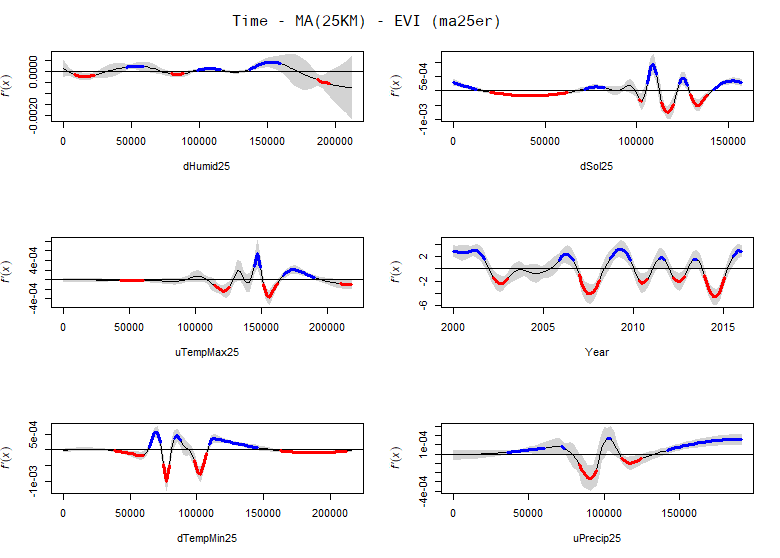
\includegraphics[width=0.8\textwidth]{ma25er.png} % first figure itself
        \caption[Model Cerrado Maranhão for 25km bandwidth using EVI values for raining season. First derivative of the trends splines from the deforestation data Generalized Additive Model (GAM)]{\textbf{Model ma25er}. Model Maranhão Cerrado for 25km bandwidth using EVI values for raining season. First derivative of the trends splines from the deforestation data Generalized Additive Model (GAM). The grey band is a 99\% simultaneous point-wise confidence interval. Sections of the spline where the confidence interval does not include zero are indicated by coloured sections. Blue colour means positive values and red colour means negative values.}
    %\end{minipage}
\end{figure}
\end{sidewaystable}

\begin{sidewaystable}
\begin{figure}[H]
 \centering
    %\begin{minipage}{1\textwidth}
        \centering
        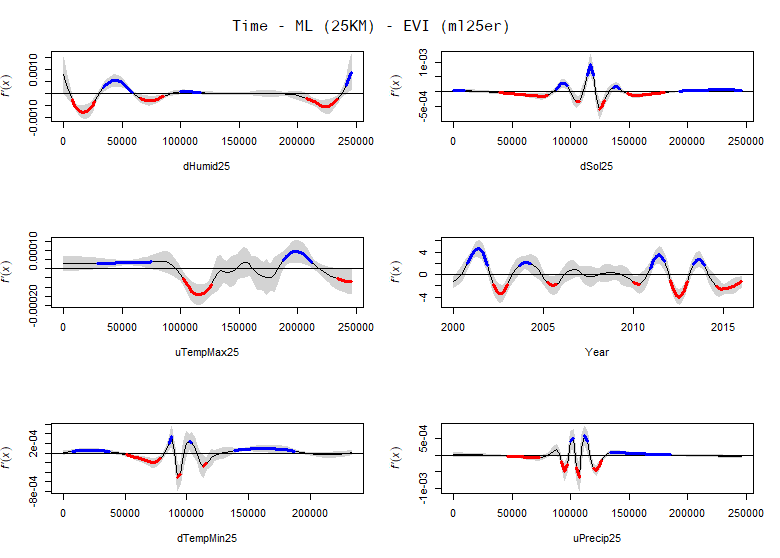
\includegraphics[width=0.8\textwidth]{ml25er.png} % second figure itself
        \caption[Model Legal Maranhão for 25km bandwidth using EVI values for raining season. First derivative of the trends splines from the deforestation data Generalized Additive Model (GAM)]{\textbf{Model lm25er}. Model Legal Maranhão for 25km bandwidth using EVI values for raining season. First derivative of the trends splines from the deforestation data Generalized Additive Model (GAM). The grey band is a 99\% simultaneous point-wise confidence interval. Sections of the spline where the confidence interval does not include zero are indicated by coloured sections. Blue colour means positive values and red colour means negative values.}
        \centering
\end{figure}
\end{sidewaystable}

%%%%%%%%%%%%%%%%%%%%%%%%%%%%%%%%%%%%%%%%%%%%%%%%%%%%%%%%%%%%%%%%%%%

\begin{sidewaystable}

\begin{figure}[H]
 \centering
    %\begin{minipage}{1\textwidth}
        \centering
        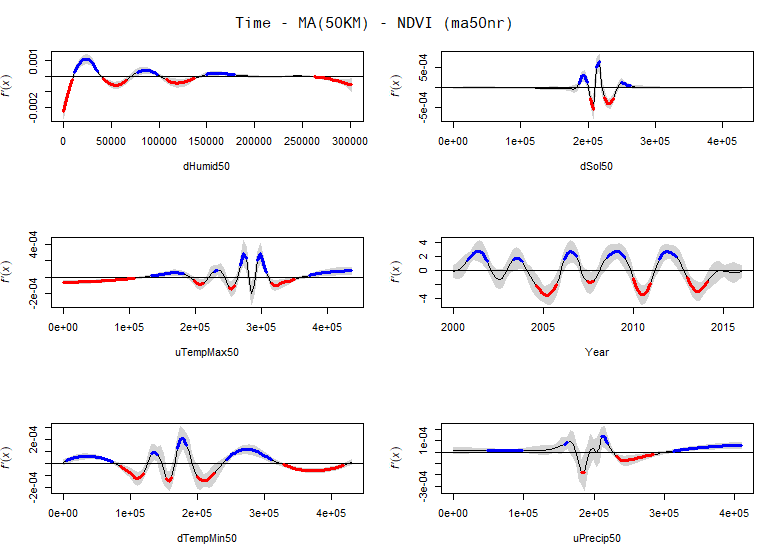
\includegraphics[width=0.8\textwidth]{ma50nr.png} % first figure itself
        \caption[Model Cerrado Maranhão for 50km bandwidth using NDVI values for raining season. First derivative of the trends splines from the deforestation data Generalized Additive Model (GAM)]{\textbf{Model ma50nr}. Model Maranhão Cerrado for 50km bandwidth using NDVI values for raining season. First derivative of the trends splines from the deforestation data Generalized Additive Model (GAM). The grey band is a 99\% simultaneous point-wise confidence interval. Sections of the spline where the confidence interval does not include zero are indicated by coloured sections. Blue colour means positive values and red colour means negative values.}
    %\end{minipage}
\end{figure}
\end{sidewaystable}

\begin{sidewaystable}

\begin{figure}[H]
 \centering
    %\begin{minipage}{1\textwidth}
        \centering
        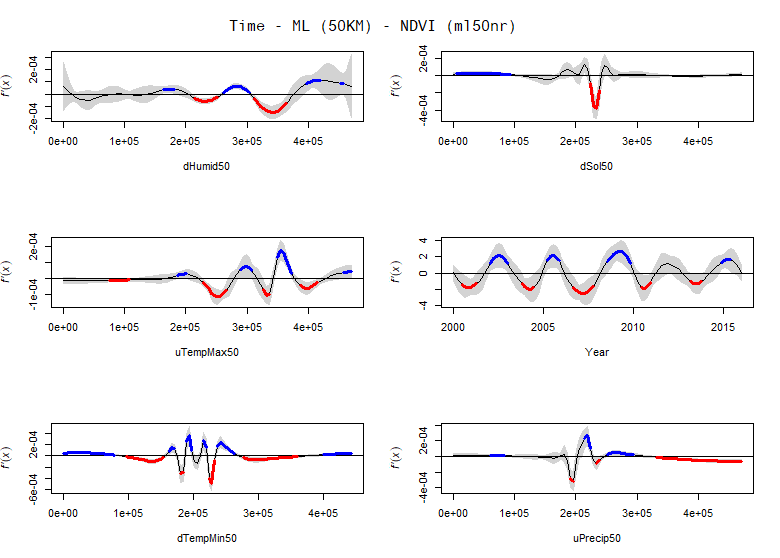
\includegraphics[width=0.8\textwidth]{ml50nr.png} % second figure itself
        \caption[Model Legal Maranhão for 50km bandwidth using NDVI values for raining season. First derivative of the trends splines from the deforestation data Generalized Additive Model (GAM)]{\textbf{Model lm50nr}. Model Legal Maranhão for 50km bandwidth using NDVI values for raining season. First derivative of the trends splines from the deforestation data Generalized Additive Model (GAM). The grey band is a 99\% simultaneous point-wise confidence interval. Sections of the spline where the confidence interval does not include zero are indicated by coloured sections. Blue colour means positive values and red colour means negative values.}
        \centering
\end{figure}
\end{sidewaystable}

\begin{sidewaystable}
\begin{figure}[H]
 \centering
    %\begin{minipage}{1\textwidth}
        \centering
        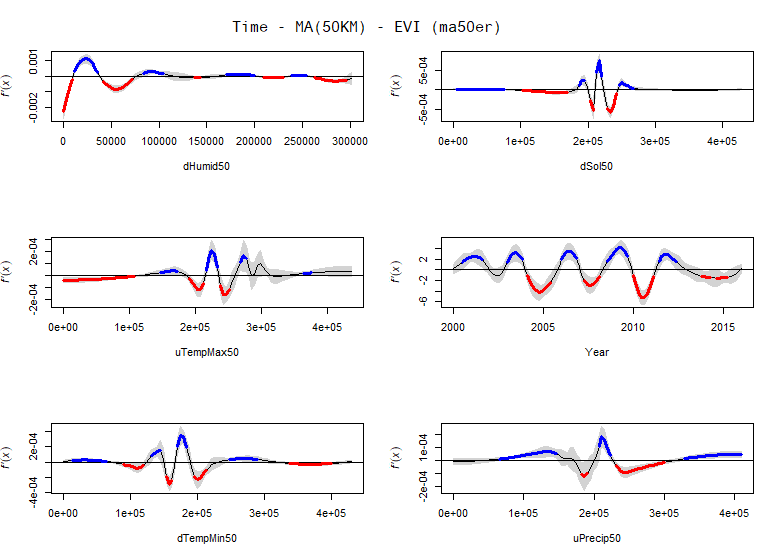
\includegraphics[width=0.8\textwidth]{ma50er.png} % first figure itself
        \caption[Model Cerrado Maranhão for 50km bandwidth using EVI values for raining season. First derivative of the trends splines from the deforestation data Generalized Additive Model (GAM)]{\textbf{Model ma50er}. Model Maranhão Cerrado for 50km bandwidth using EVI values for raining season. First derivative of the trends splines from the deforestation data Generalized Additive Model (GAM). The grey band is a 99\% simultaneous point-wise confidence interval. Sections of the spline where the confidence interval does not include zero are indicated by coloured sections. Blue colour means positive values and red colour means negative values.}
    %\end{minipage}
\end{figure}
\end{sidewaystable}

\begin{sidewaystable}


\begin{figure}[H]
 \centering
    %\begin{minipage}{1\textwidth}
        \centering
        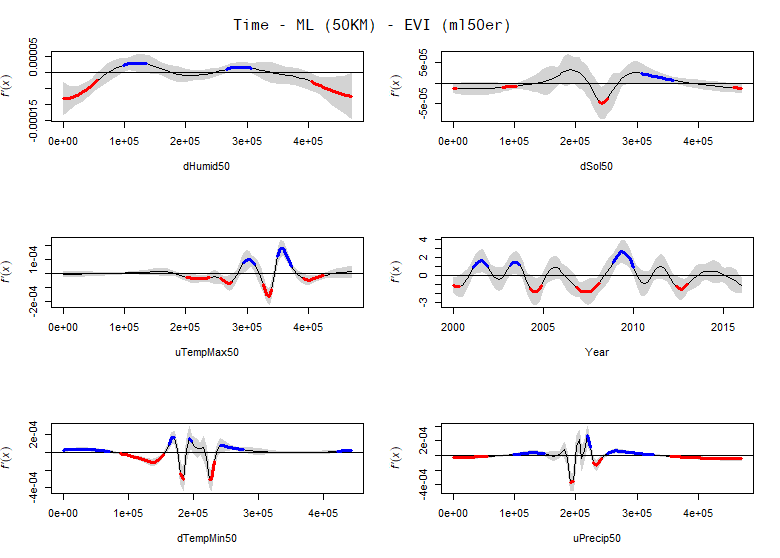
\includegraphics[width=0.8\textwidth]{ml50er.png} % second figure itself
        \caption[Model Legal Maranhão for 50km bandwidth using EVI values for raining season. First derivative of the trends splines from the deforestation data Generalized Additive Model (GAM)]{\textbf{Model lm50er}. Model Legal Maranhão for 50km bandwidth using EVI values for raining season. First derivative of the trends splines from the deforestation data Generalized Additive Model (GAM). The grey band is a 99\% simultaneous point-wise confidence interval. Sections of the spline where the confidence interval does not include zero are indicated by coloured sections. Blue colour means positive values and red colour means negative values.}
        \centering
\end{figure}
\end{sidewaystable}

%%%%%%%%%%%%%%%%%%%%%%%%%%%%%%%%%%%%%%%%%%%%%%%%%%%%%%%%%%%%%%%%%%%%%%%%%%%
\begin{sidewaystable}

\begin{figure}[H]
 \centering
    %\begin{minipage}{1\textwidth}
        \centering
        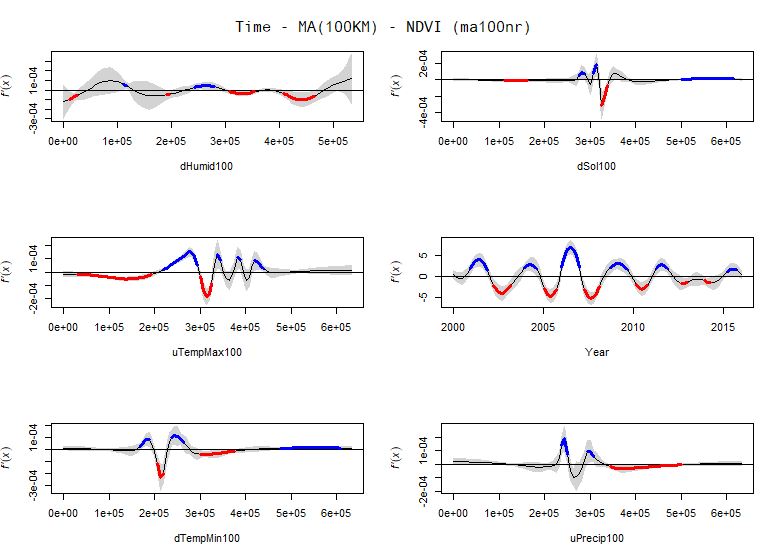
\includegraphics[width=0.8\textwidth]{ma100nr.png} % first figure itself
        \caption[Model Cerrado Maranhão for 100km bandwidth using NDVI values for raining season. First derivative of the trends splines from the deforestation data Generalized Additive Model (GAM)]{\textbf{Model ma100nr}. Model Maranhão Cerrado for 100km bandwidth using NDVI values for raining season. First derivative of the trends splines from the deforestation data Generalized Additive Model (GAM). The grey band is a 99\% simultaneous point-wise confidence interval. Sections of the spline where the confidence interval does not include zero are indicated by coloured sections. Blue colour means positive values and red colour means negative values.}
    %\end{minipage}
\end{figure}
\end{sidewaystable}

\begin{sidewaystable}

\begin{figure}[H]
 \centering
    %\begin{minipage}{1\textwidth}
        \centering
        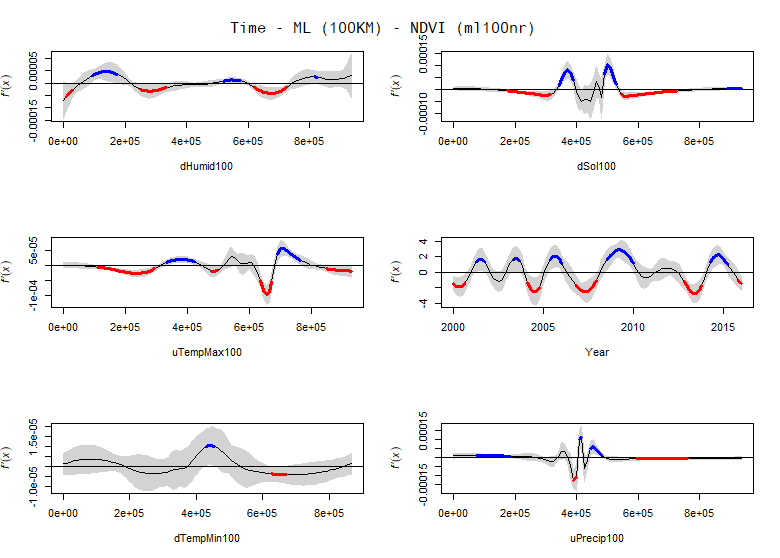
\includegraphics[width=0.8\textwidth]{ml100nr.png} % second figure itself
        \caption[Model Legal Maranhão for 100km bandwidth using NDVI values for raining season. First derivative of the trends splines from the deforestation data Generalized Additive Model (GAM)]{\textbf{Model lm100nr}. Model Legal Maranhão for 100km bandwidth using NDVI values for raining season. First derivative of the trends splines from the deforestation data Generalized Additive Model (GAM). The grey band is a 99\% simultaneous point-wise confidence interval. Sections of the spline where the confidence interval does not include zero are indicated by coloured sections. Blue colour means positive values and red colour means negative values.}
        \centering
\end{figure}
\end{sidewaystable}

\begin{sidewaystable}

\begin{figure}[H]
 \centering
    %\begin{minipage}{1\textwidth}
        \centering
        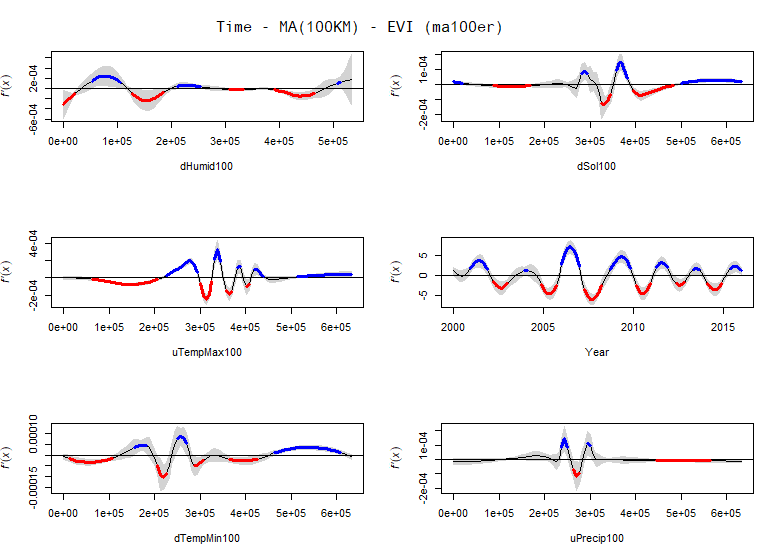
\includegraphics[width=0.8\textwidth]{ma100er.png} % first figure itself
        \caption[Model Cerrado Maranhão for 100km bandwidth using EVI values for raining season. First derivative of the trends splines from the deforestation data Generalized Additive Model (GAM)]{\textbf{Model ma100er}. Model Maranhão Cerrado for 100km bandwidth using EVI values for raining season. First derivative of the trends splines from the deforestation data Generalized Additive Model (GAM). The grey band is a 99\% simultaneous point-wise confidence interval. Sections of the spline where the confidence interval does not include zero are indicated by coloured sections. Blue colour means positive values and red colour means negative values.}
    %\end{minipage}
\end{figure}
\end{sidewaystable}

\begin{sidewaystable}

\begin{figure}[H]
 \centering
    %\begin{minipage}{1\textwidth}
        \centering
        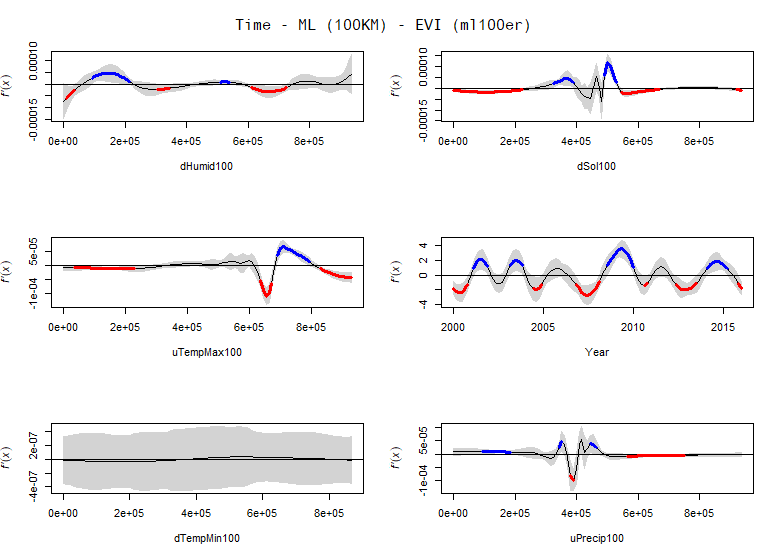
\includegraphics[width=0.8\textwidth]{ml100er.png} % second figure itself
        \caption[Model Legal Maranhão for 100km bandwidth using EVI values for raining season. First derivative of the trends splines from the deforestation data Generalized Additive Model (GAM)]{\textbf{Model lm100er}. Model Legal Maranhão for 100km bandwidth using EVI values for raining season. First derivative of the trends splines from the deforestation data Generalized Additive Model (GAM). The grey band is a 99\% simultaneous point-wise confidence interval. Sections of the spline where the confidence interval does not include zero are indicated by coloured sections. Blue colour means positive values and red colour means negative values.}
        \centering
\end{figure}
\end{sidewaystable}
%%%%%%%%%%%%%%%%%%%%%%%%%%%%%% D R Y %%%%%%%%%%%%%%%%%%%%%%%%%%%%%%%%%%%%%%%%%%

\begin{sidewaystable}

\begin{figure}[H]
 \centering
    %\begin{minipage}{1\textwidth}
        \centering
        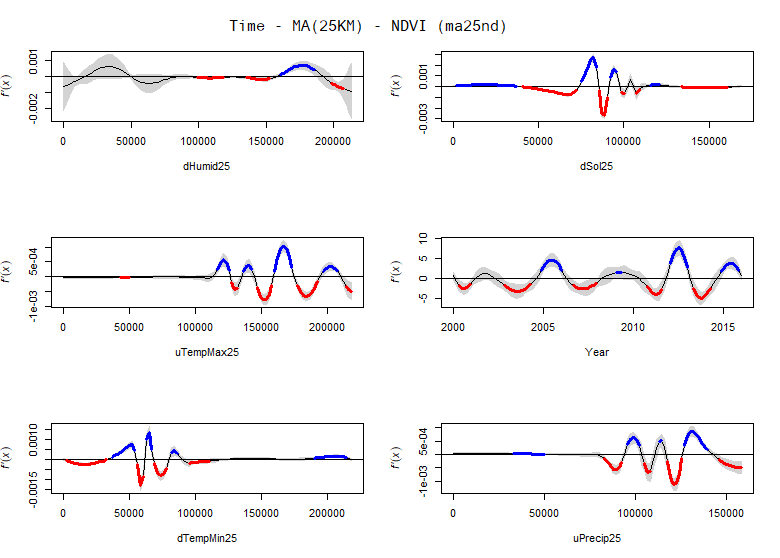
\includegraphics[width=0.8\textwidth]{ma25nd.png} % first figure itself
        \caption[Model Cerrado Maranhão for 25km bandwidth using NDVI values for dry season. First derivative of the trends splines from the deforestation data Generalized Additive Model (GAM)]{\textbf{Model ma25nd}. Model Maranhão Cerrado for 25km bandwidth using NDVI values for dry season. First derivative of the trends splines from the deforestation data Generalized Additive Model (GAM). The grey band is a 99\% simultaneous point-wise confidence interval. Sections of the spline where the confidence interval does not include zero are indicated by coloured sections. Blue colour means positive values and red colour means negative values.}
    %\end{minipage}
\end{figure}
\end{sidewaystable}

\begin{sidewaystable}


\begin{figure}[H]
 \centering
    %\begin{minipage}{1\textwidth}
        \centering
        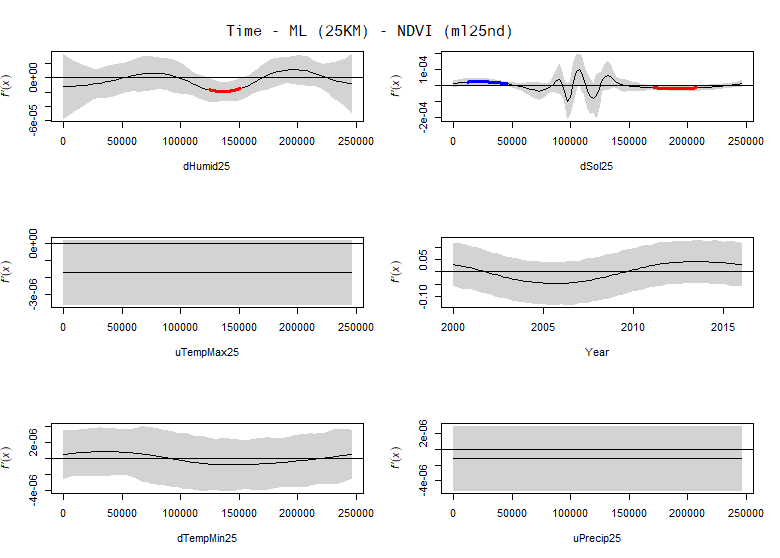
\includegraphics[width=0.8\textwidth]{ml25nd.png} % second figure itself
        \caption[Model Legal Maranhão for 25km bandwidth using NDVI values for dry season. First derivative of the trends splines from the deforestation data Generalized Additive Model (GAM)]{\textbf{Model lm25nd}. Model Legal Maranhão for 25km bandwidth using NDVI values for dry season. First derivative of the trends splines from the deforestation data Generalized Additive Model (GAM). The grey band is a 99\% simultaneous point-wise confidence interval. Sections of the spline where the confidence interval does not include zero are indicated by coloured sections. Blue colour means positive values and red colour means negative values.}
        \centering
\end{figure}
\end{sidewaystable}

\begin{sidewaystable}

\begin{figure}[H]
 \centering
    %\begin{minipage}{1\textwidth}
        \centering
        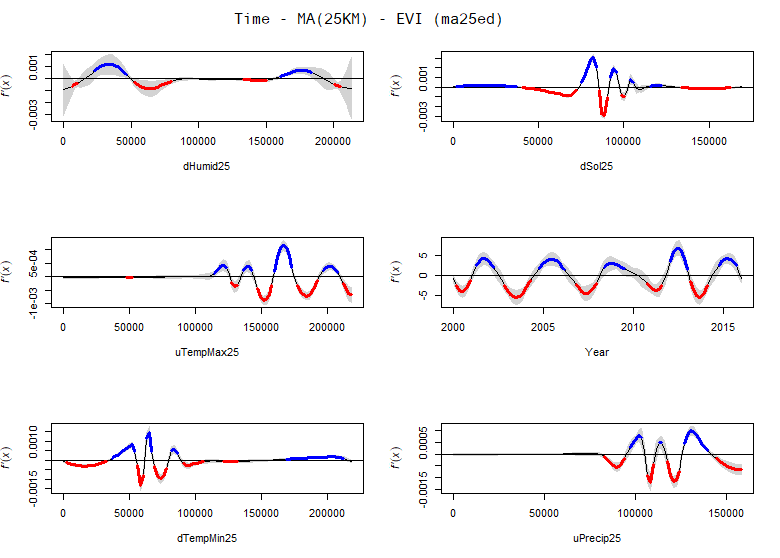
\includegraphics[width=0.8\textwidth]{ma25ed.png} % first figure itself
        \caption[Model Cerrado Maranhão for 25km bandwidth using EVI values for dry season. First derivative of the trends splines from the deforestation data Generalized Additive Model (GAM)]{\textbf{Model ma25ed}. Model Maranhão Cerrado for 25km bandwidth using EVI values for dry season. First derivative of the trends splines from the deforestation data Generalized Additive Model (GAM). The grey band is a 99\% simultaneous point-wise confidence interval. Sections of the spline where the confidence interval does not include zero are indicated by coloured sections. Blue colour means positive values and red colour means negative values.}
    %\end{minipage}
\end{figure}
\end{sidewaystable}

\begin{sidewaystable}

\begin{figure}[H]
 \centering
    %\begin{minipage}{1\textwidth}
        \centering
        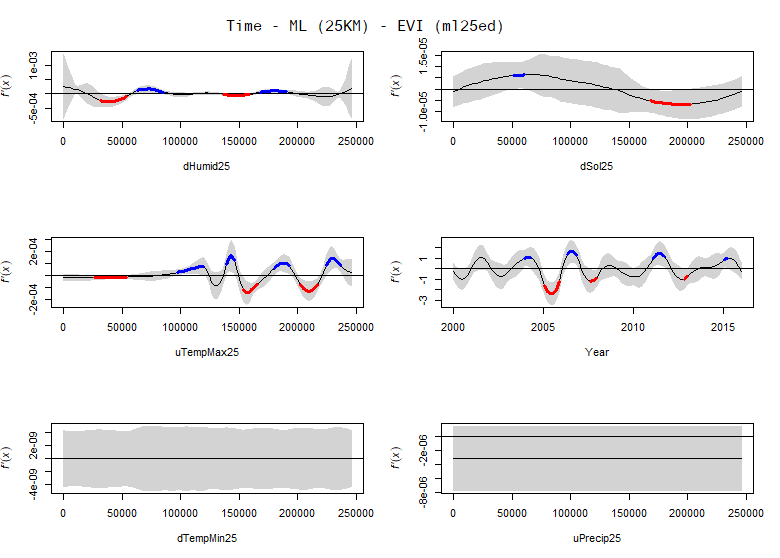
\includegraphics[width=0.8\textwidth]{ml25ed.png} % second figure itself
        \caption[Model Legal Maranhão for 25km bandwidth using EVI values for dry season. First derivative of the trends splines from the deforestation data Generalized Additive Model (GAM)]{\textbf{Model lm25ed}. Model Legal Maranhão for 25km bandwidth using EVI values for dry season. First derivative of the trends splines from the deforestation data Generalized Additive Model (GAM). The grey band is a 99\% simultaneous point-wise confidence interval. Sections of the spline where the confidence interval does not include zero are indicated by coloured sections. Blue colour means positive values and red colour means negative values.}
        \centering
\end{figure}
\end{sidewaystable}
%%%%%%%%%%%%%%%%%%%%%%%%%%%%%%%%%%%%%%%%%%%%%%%%%%%%%%%%%%%%%%%%%%%%%%%%%%%%%%
\begin{sidewaystable}

\begin{figure}[H]
 \centering
    %\begin{minipage}{1\textwidth}
        \centering
        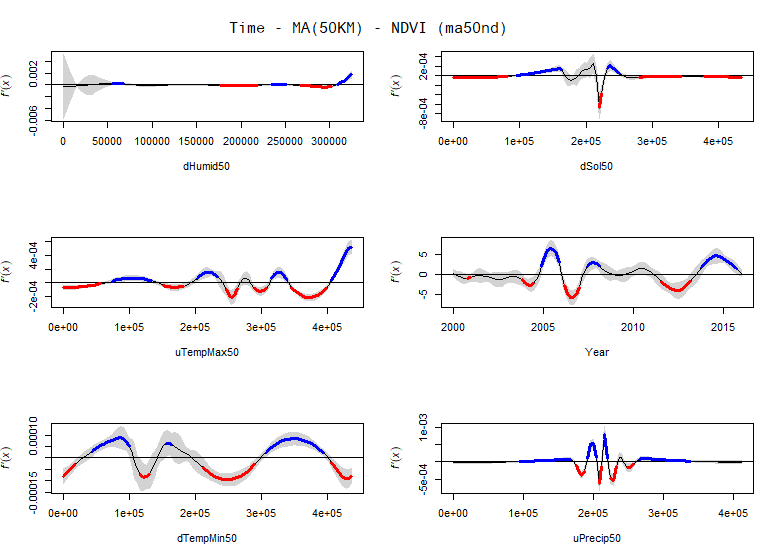
\includegraphics[width=0.8\textwidth]{ma50nd.png} % first figure itself
        \caption[Model Cerrado Maranhão for 50km bandwidth using NDVI values for dry season. First derivative of the trends splines from the deforestation data Generalized Additive Model (GAM)]{\textbf{Model ma50nd}. Model Maranhão Cerrado for 50km bandwidth using NDVI values for dry season. First derivative of the trends splines from the deforestation data Generalized Additive Model (GAM). The grey band is a 99\% simultaneous point-wise confidence interval. Sections of the spline where the confidence interval does not include zero are indicated by coloured sections. Blue colour means positive values and red colour means negative values.}
    %\end{minipage}
\end{figure}
\end{sidewaystable}

\begin{sidewaystable}

\begin{figure}[H]
 \centering
    %\begin{minipage}{1\textwidth}
        \centering
        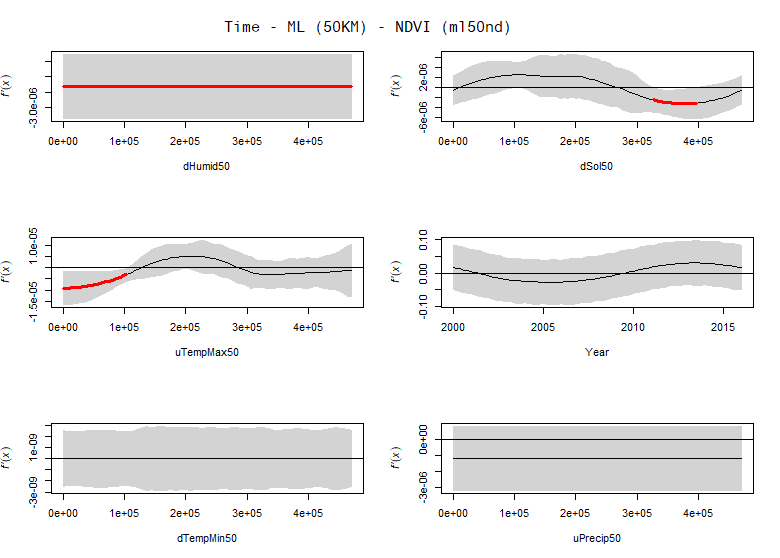
\includegraphics[width=0.8\textwidth]{ml50nd.png} % second figure itself
        \caption[Model Legal Maranhão for 50km bandwidth using NDVI values for dry season. First derivative of the trends splines from the deforestation data Generalized Additive Model (GAM)]{\textbf{Model lm50nd}. Model Legal Maranhão for 50km bandwidth using NDVI values for dry season. First derivative of the trends splines from the deforestation data Generalized Additive Model (GAM). The grey band is a 99\% simultaneous point-wise confidence interval. Sections of the spline where the confidence interval does not include zero are indicated by coloured sections. Blue colour means positive values and red colour means negative values.}
        \centering
\end{figure}
\end{sidewaystable}

\begin{sidewaystable}

\begin{figure}[H]
 \centering
    %\begin{minipage}{1\textwidth}
        \centering
        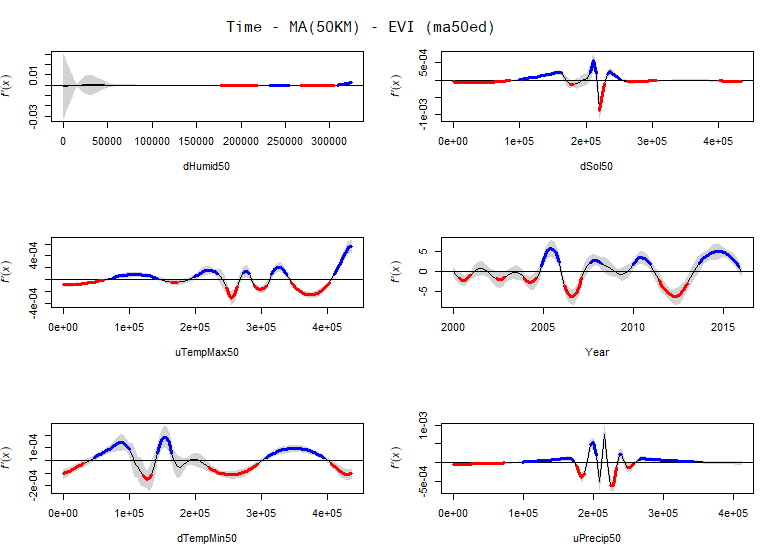
\includegraphics[width=0.8\textwidth]{ma50ed.png} % first figure itself
        \caption[Model Cerrado Maranhão for 50km bandwidth using EVI values for dry season. First derivative of the trends splines from the deforestation data Generalized Additive Model (GAM)]{\textbf{Model ma50ed}. Model Maranhão Cerrado for 50km bandwidth using EVI values for dry season. First derivative of the trends splines from the deforestation data Generalized Additive Model (GAM). The grey band is a 99\% simultaneous point-wise confidence interval. Sections of the spline where the confidence interval does not include zero are indicated by coloured sections. Blue colour means positive values and red colour means negative values.}
    %\end{minipage}
\end{figure}
\end{sidewaystable}

\begin{sidewaystable}

\begin{figure}[H]
 \centering
    %\begin{minipage}{1\textwidth}
        \centering
        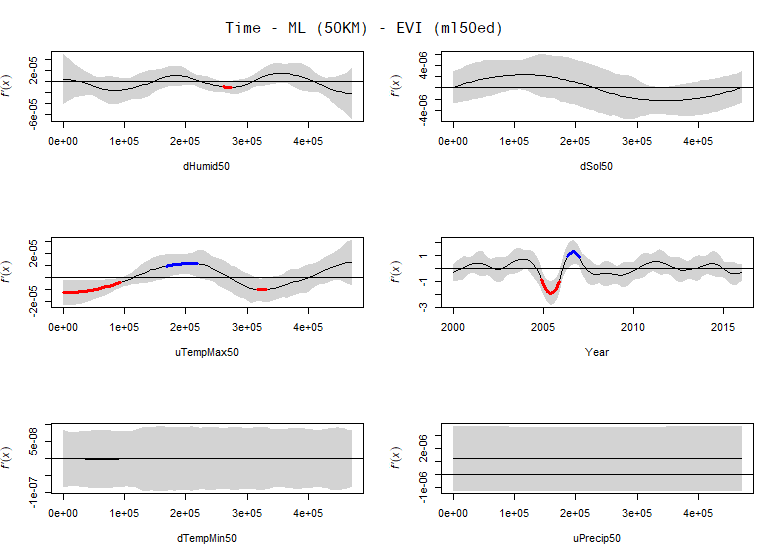
\includegraphics[width=0.8\textwidth]{ml50ed.png} % second figure itself
        \caption[Model Legal Maranhão for 50km bandwidth using EVI values for dry season. First derivative of the trends splines from the deforestation data Generalized Additive Model (GAM)]{\textbf{Model lm50ed}. Model Legal Maranhão for 50km bandwidth using EVI values for dry season. First derivative of the trends splines from the deforestation data Generalized Additive Model (GAM). The grey band is a 99\% simultaneous point-wise confidence interval. Sections of the spline where the confidence interval does not include zero are indicated by coloured sections. Blue colour means positive values and red colour means negative values.}
        \centering
\end{figure}
\end{sidewaystable}
%%%%%%%%%%%%%%%%%%%%%%%%%%%%%%%%%%%%%%%%%%%%%%%%%%%%%%%%%%%%%%%%%%%%%%%%%%%%%%%
\begin{sidewaystable}


\begin{figure}[H]
 \centering
    %\begin{minipage}{1\textwidth}
        \centering
        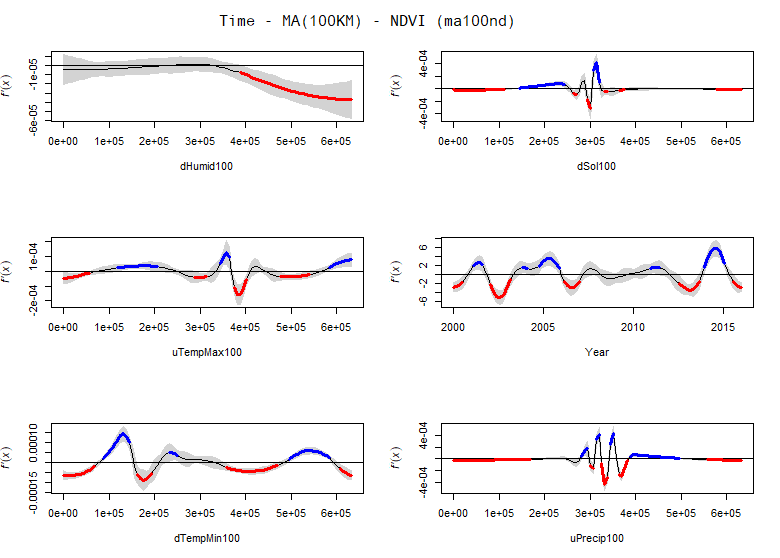
\includegraphics[width=0.8\textwidth]{ma100nd.png} % first figure itself
        \caption[Model Cerrado Maranhão for 100km bandwidth using NDVI values for dry season. First derivative of the trends splines from the deforestation data Generalized Additive Model (GAM)]{\textbf{Model ma100nd}. Model Maranhão Cerrado for 100km bandwidth using NDVI values for dry season. First derivative of the trends splines from the deforestation data Generalized Additive Model (GAM). The grey band is a 99\% simultaneous point-wise confidence interval. Sections of the spline where the confidence interval does not include zero are indicated by coloured sections. Blue colour means positive values and red colour means negative values.}
    %\end{minipage}
\end{figure}
\end{sidewaystable}

\begin{sidewaystable}

\begin{figure}[H]
 \centering
    %\begin{minipage}{1\textwidth}
        \centering
        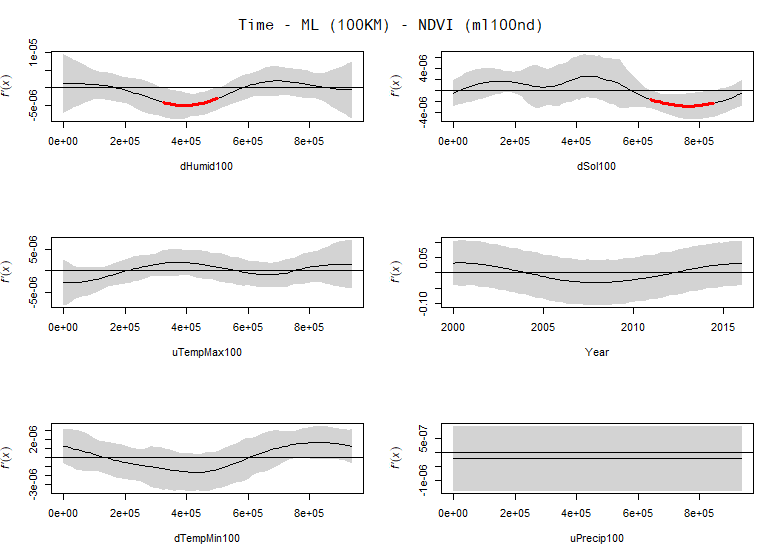
\includegraphics[width=0.8\textwidth]{ml100nd.png} % second figure itself
        \caption[Model Legal Maranhão for 100km bandwidth using NDVI values for dry season. First derivative of the trends splines from the deforestation data Generalized Additive Model (GAM)]{\textbf{Model lm100nd}. Model Legal Maranhão for 100km bandwidth using NDVI values for dry season. First derivative of the trends splines from the deforestation data Generalized Additive Model (GAM). The grey band is a 99\% simultaneous point-wise confidence interval. Sections of the spline where the confidence interval does not include zero are indicated by coloured sections. Blue colour means positive values and red colour means negative values.}
        \centering
\end{figure}
\end{sidewaystable}

\begin{sidewaystable}


\begin{figure}[H]
 \centering
    %\begin{minipage}{1\textwidth}
        \centering
        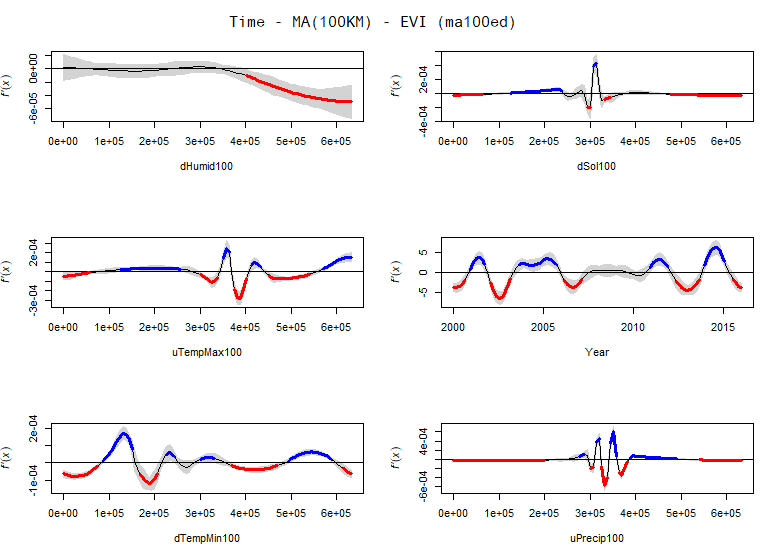
\includegraphics[width=0.8\textwidth]{ma100ed.png} % first figure itself
        \caption[Model Cerrado Maranhão for 100km bandwidth using EVI values for dry season. First derivative of the trends splines from the deforestation data Generalized Additive Model (GAM)]{\textbf{Model ma100ed}. Model Maranhão Cerrado for 100km bandwidth using EVI values for dry season. First derivative of the trends splines from the deforestation data Generalized Additive Model (GAM). The grey band is a 99\% simultaneous point-wise confidence interval. Sections of the spline where the confidence interval does not include zero are indicated by coloured sections. Blue colour means positive values and red colour means negative values.}
    %\end{minipage}
\end{figure}
\end{sidewaystable}

\begin{sidewaystable}

\begin{figure}[H]
 \centering
    %\begin{minipage}{1\textwidth}
        \centering
        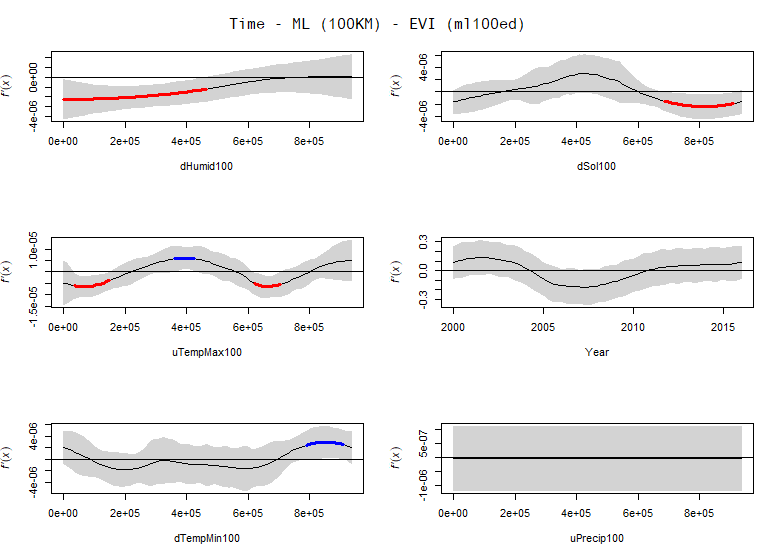
\includegraphics[width=0.8\textwidth]{ml100ed.png} % second figure itself
        \caption[Model Legal Maranhão for 100km bandwidth using EVI values for dry season. First derivative of the trends splines from the deforestation data Generalized Additive Model (GAM)]{\textbf{Model lm100ed}. Model Legal Maranhão for 100km bandwidth using EVI values for dry season. First derivative of the trends splines from the deforestation data Generalized Additive Model (GAM). The grey band is a 99\% simultaneous point-wise confidence interval. Sections of the spline where the confidence interval does not include zero are indicated by coloured sections. Blue colour means positive values and red colour means negative values.}
        \centering
\end{figure}
\end{sidewaystable}


\begin{figure}[H]
  \centering
  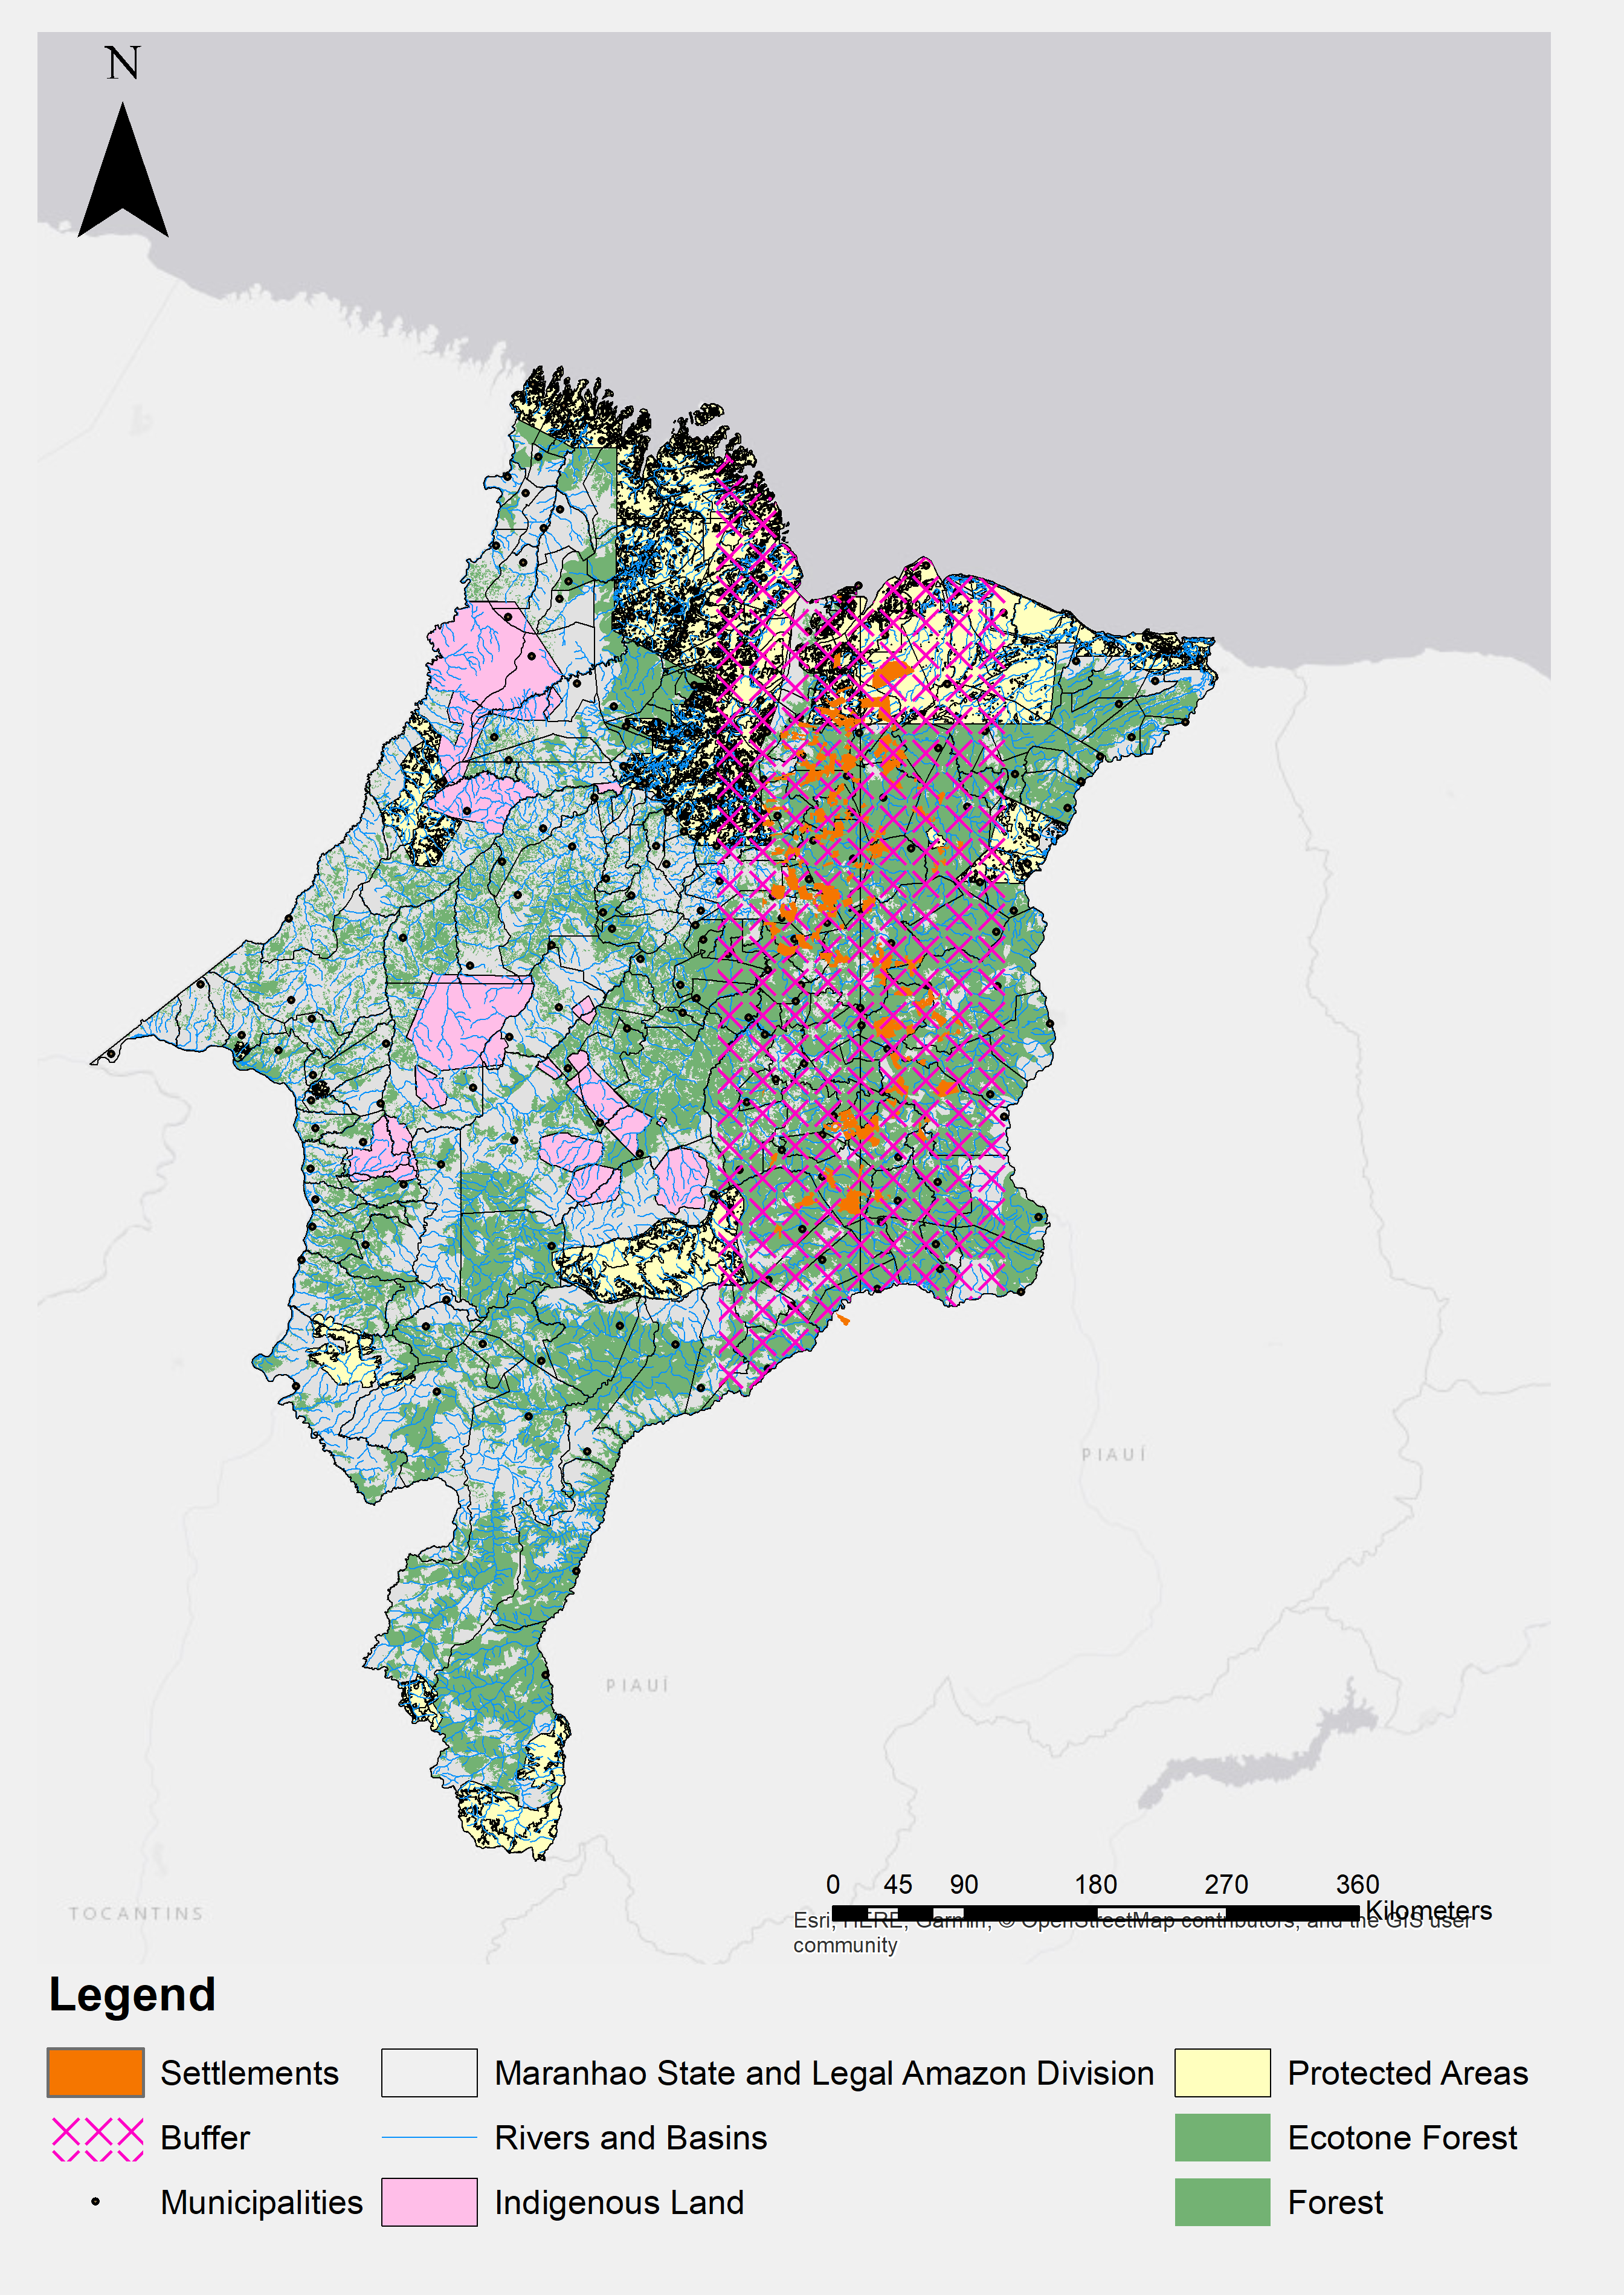
\includegraphics[width=1\textwidth]{Chapter2/MaranhaoChapter2_Fig3.png}
\caption[Maranhão state and Settlements]{Maranhão State and the Legal Amazon delimitation with buffers of 100km and the presence of settlements within the buffer. The map includes municipalities centre, rivers and basins, protected areas and indigenous land. Source: \citep{MMMAwebsite,nugeo_2018,embrapa_2018, INCRA}.}
\label{fig:delimitacaosett2}
\end{figure}




\begin{sidewaystable}


\begin{figure}[H]
  \centering
  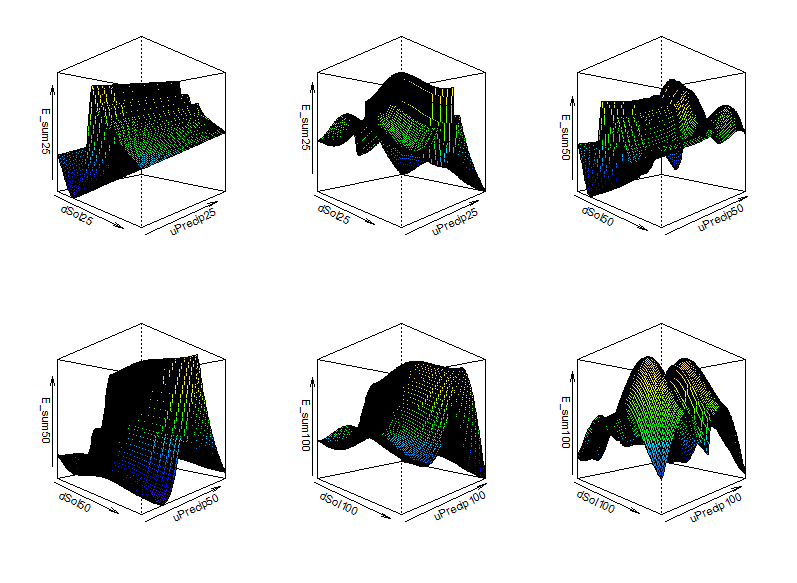
\includegraphics[width=0.85\textwidth, inner]{visgam.png}
\caption[Interactions of variables and the Baseline model for bandwidth of 25km, 50km and, 100km]{Interactions of variables and the Baseline model for bandwidth of 25km, 50km and, 100km.}
\label{fig:visgam}
\end{figure}
\end{sidewaystable}

\begin{sidewaystable}

\begin{figure}[H]
  \centering
  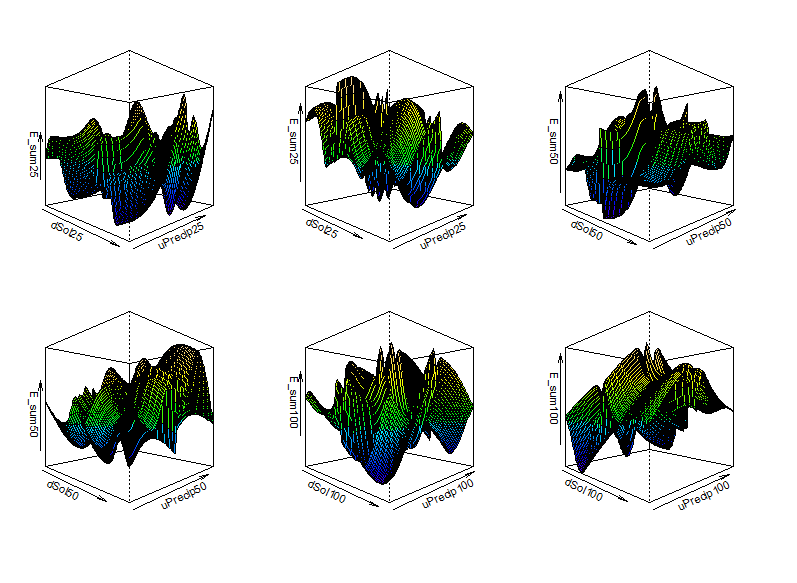
\includegraphics[width=0.85\textwidth, inner]{visgamr.png}
\caption[Interactions of variables and the Baseline model for bandwidth of 25km, 50km and, 100km in the raining season]{Interactions of variables and the Baseline model for bandwidth of 25km, 50km and, 100km in the raining season. }
\label{fig:visgamr}
\end{figure}
\end{sidewaystable}

\begin{sidewaystable}

\begin{figure}[H]
  \centering
  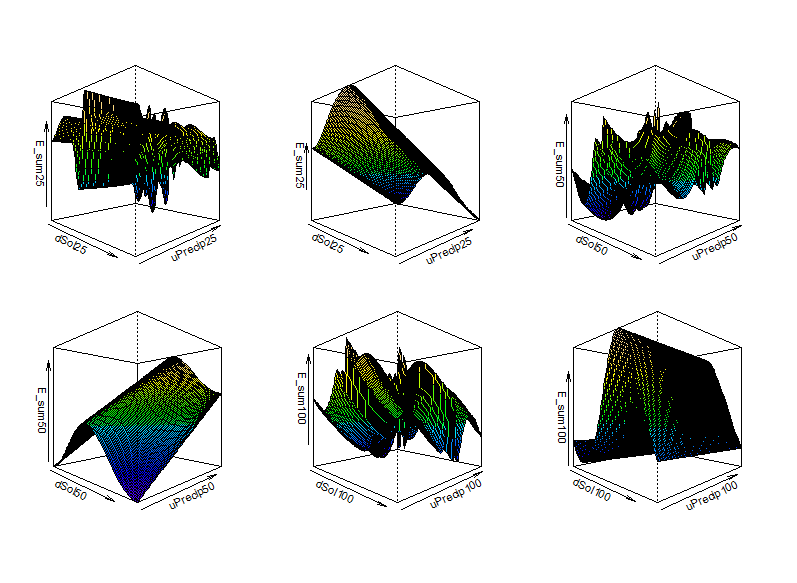
\includegraphics[width=0.85\textwidth, inner]{visgamd.png}
\caption[Interactions of variables and the Baseline model for bandwidth of 25km, 50km and, 100km in the dry season]{Interactions of variables and the Baseline model for bandwidth of 25km, 50km and, 100km in the dry season.}
\label{fig:visgamd}
\end{figure}
\end{sidewaystable}

\begin{sidewaystable}

\begin{figure}[H]
  \centering
  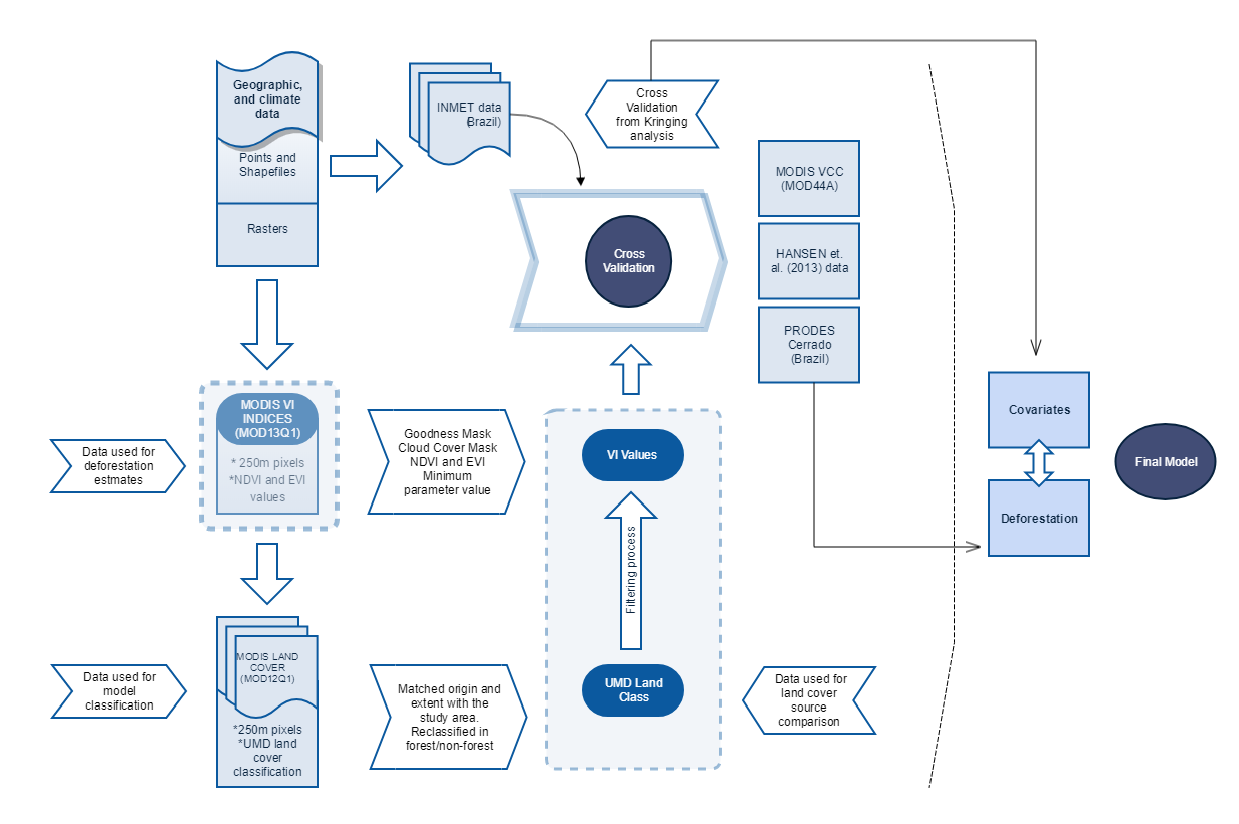
\includegraphics[width=0.9\textwidth, inner]{method.png}
\caption[Flowchart of method applied to data]{Flowchart of method applied to data . Moving from left to right indicates increasing levels of data processing during the study.}
\label{fig:method2}
\end{figure}
\end{sidewaystable}


